\documentclass[titlepage,a4paper]{article}

\usepackage{a4wide}
\usepackage[colorlinks=true,linkcolor=black,urlcolor=blue,bookmarksopen=true]{hyperref}
\usepackage{bookmark}
\usepackage{fancyhdr}
\usepackage[spanish]{babel}
\usepackage[utf8]{inputenc}
\usepackage[T1]{fontenc}
\usepackage{graphicx}
\usepackage{float}
\usepackage{amsfonts}
\usepackage{minted} 

\pagestyle{fancy} % Encabezado y pie de página
\fancyhf{}
\fancyhead[L]{Resumen}
\fancyhead[R]{Organización de datos - FIUBA}
\renewcommand{\headrulewidth}{0.4pt}
\fancyfoot[C]{\thepage}
\renewcommand{\footrulewidth}{0.4pt}

\begin{document}
\begin{titlepage} % Carátula
	\hfill
\includegraphics[width=6cm]{imagenesResumen/logofiuba.jpg}
    \centering
    \vfill
    \Huge \textbf{Resumen Datos}
    \vskip2cm
    \Large Organización de datos, Curso Collinet - FIUBA\\
    \vfill
    \begin{tabular}{ | l | l | }
      \hline
       Grassano, Bruno &  bgrassano@fi.uba.ar \\ \hline
  	\end{tabular}
    \vfill
    \vfill
\end{titlepage}

\tableofcontents % Índice general
\newpage

\section{Introducción}\label{sec:intro}
El presente archivo es un resumen que recopila el contenido dado en la materia Organización de datos, Curso Collinet 2C2020. Lo fui armando con los diferentes apuntes que tome durante las clases, contenido presentado durante las mismas, y en algunos casos busque algo mas de información para completar.

\section{Análisis Exploratorio}
Es un enfoque que comprende un conjunto de tareas para analizar conjuntos de datos, de forma tal de encontrar sus principales características.

Se comienza siempre formulando una pregunta interesante, se reúnen los datos, y se desarrolla el proceso necesario para poder responderla.

\subsection{Feature Engineering}
Forma a través de la cual se van tratando los datos. Comprende conversiones de tipos, missings, selección, creación de nuevas variables a partir de las que ya tenemos y reducciones dimensionales.

\begin{center}
    \textit{Good features allow a simple model to beat a complex model.}
    
    \textit{Peter Norving}
\end{center}

\subsubsection{Conversión}
Los modelos entienden números, por lo que es necesario convertir los atributos a variables numéricas.



\subsubsection*{Variables categóricas}
\begin{itemize}
    \item One Hot Encoding: Por cada variable categórica crea una binaria. Tener cuidado con el problema de la colinealidad. Solución, crear para todos menos una la variable binaria. La ausencia de todas significa que se esta en presencia de la no codificada.
    \item Bin Counting Scheme: Convierte los valores categóricos en probabilidades. Útil para cuando se tiene muchas categorías.
    \item Hashing Trick: Mapea de un dominio muchísimo mayor a uno mas acotado. Muy bueno también para cuando se tienen muchas categorías. Se utiliza una funcion hash para conseguirlo.
\end{itemize}

Si se quiere conservar algun orden en particular, se puede utilizar Ordinal Encoder. Tener cuidado de que no se de el caso de agregar un orden donde no corresponda. \textit{Ej. Azul < Rojo}


\subsubsection{Missing values}
\subsubsection*{Missing completely at random}
En este caso la probabilidad de que un valor sea missing es la misma para todas las instancias. En este caso no depende de las medidas de otras variables. No tiene sentido intentar adivinar este caso. \textit{Ej. Respuesta de una encuesta}

\subsubsection*{Missing at random}
La probabilidad de missing depende de información que si tengo. \textit{Ej. Edad relacionado con si una persona vive. Si no vive, y no tengo cargado el valor de edad ahí esta relacionado.}

\subsubsection*{Missing not at random}
La probabilidad de missing esta relacionada con los valores perdidos. \textit{Ej. La edad quizás prefieren no decirla, o el sueldo si es alto también.}

\subsubsection*{Soluciones}
\begin{itemize}
    \item Utilizar algoritmos que acepten datos faltantes.
    \item Eliminar los datos con problemas. ¿Filas? ¿Columnas? ¿Esta bien borrarlo? Depende siempre del caso.
    \item Convertir el valor faltante en una categoría. \textit{Ej. No responde}.
    \item Rellenar el valor faltante con algún criterio. \textit{Ej. Media, mediana, moda, etc} En estos casos puede convenir agregar una columna indicadora de que ese valor fue rellenado. Esto puede hacer que se le asigne menos peso al momento de mirarlo.
\end{itemize}

\subsubsection{Selección}
Esto busca reducir la dimensión mediante la eliminación de variables poco útiles. Favorece a la generalización y puede acelerar la velocidad del modelo mientras que mejora su interpretabilidad.

\subsubsection*{Técnicas}
\begin{itemize}
    \item Filter: Se realiza un ranking de cada variable generado a través de algún método estadístico. Se busca encontrar que variable afecta mas el valor a predecir.
    \item Wrapper: Encapsula la funcionalidad. Trata al problema de selección como una busqueda, ya que trata de conseguir la mejor combinación de variables. (Alto tiempo de computo). Tiene forward selection, backward selection, y random selection. Se puede utilizar también cualquier método que trabaje con problemas de combinatoria. \textit{Ej Forward: Selecciono 1 al azar. Selecciono 2, ¿Mejoro?, selecciono mas y sigo preguntando.}
    \item Embedded: Rankea las variables segun métodos internos de cada algoritmo. Busca determinar cual es mas importante para predecir. \textit{Ej. Lasso, Ridge, Elastic Net}. Ver \ref{regularizaciones}
\end{itemize}

\subsection{Visualización}
\begin{itemize}
    \item Para entender el trabajo y comunicarlo.
    \item Entender de forma mas rápida y eficiente.
    \item Comunicarlo de forma concisa y clara.
    \item Permite encontrar patrones y relaciones.
    \item Existe una amplia variedad de tipos de gráficos, cada uno con su objetivo.
\end{itemize}

Pagina con varios tipos de \href{https://www.python-graph-gallery.com/}{gráficos}.

\newpage

\section{Clustering}

Métodos de aprendizaje no supervisado. No se sabe que resultado esperar. Lo que hace es juntar los datos para ver como están relacionados.

Su objetivo es encontrar grupos de instancias similares entre si. Depende mucho de la naturaleza de los datos.


\subsection{K-Means}
Algoritmo que busca minimizar la ecuación de distorsión de clustering. Tengo los datos en $p$ dimensiones.

\subsubsection*{Algoritmo}
\begin{enumerate}
    \item Elegir k centroides al azar.
    \item Asignar cada instancia al centroide mas cercano.
    \item Recomputar el centroide de cada cluster.
    \item Repetir paso 2 y 3 hasta que los centroides no cambien.
\end{enumerate}


\subsubsection*{Fortalezas}
\begin{itemize}
    \item Simple
    \item Eficiente
    \item Escala muy bien
\end{itemize}

\subsubsection*{Debilidades}
\begin{itemize}
    \item Especificar K
    \item Sensible a ruido
    \item Muy sensible a la elección de centroides iniciales.
    \item Solo encuentra clusters globulares.
\end{itemize}


\begin{figure}[!htb]
    \centering
    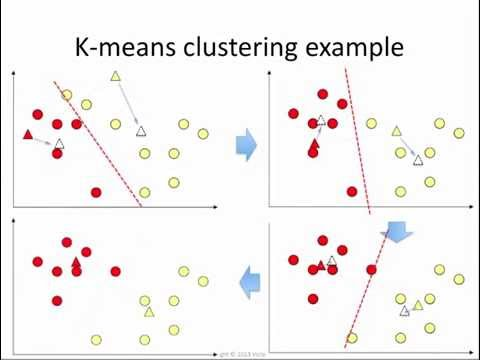
\includegraphics[width=0.5\textwidth]{imagenesResumen/K-Means.jpg}
    \caption{Ejemplo de K-Means, notar como se va moviendo el centroide.}
\end{figure}

\newpage

\subsection{Clustering Jerárquico Aglomerativo}
\subsubsection*{Notas}
\begin{itemize}
    \item Cada instancia comienza en un cluster distinto.
    \item Cada instancia se va uniendo con el mas cercano.
    \item Bottom up
\end{itemize}

\subsubsection*{Fortalezas}
\begin{itemize}
    \item No tiene K
    \item Se reproduce una representación jerárquica (Dendograma)
\end{itemize}

\subsubsection*{Debilidades}
\begin{itemize}
    \item No busca optimizar una función
    \item Sensible a ruido
\end{itemize}

\begin{figure}[!htb]
    \centering
    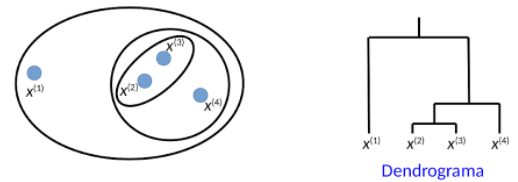
\includegraphics[width=0.7\textwidth]{imagenesResumen/ClusteringJerarquicoAglomerativo.PNG}
    \caption{Ejemplo de Clustering Jerarquico Aglomerativo.}
\end{figure}

\subsection{Clustering Jerárquico Divisivo}
Similar al anterior en cuanto a procedimiento, solo que se comienza todo junto y se va dividiendo a medida que se va bajando.

\subsection{DBSCAN}
Se busca conseguir una mejora al ahorrar una cantidad de pasos en el algoritmo.

\begin{itemize}
    \item \textbf{CORE POINTS} Son los puntos que tienen una densidad alta
    \item \textbf{BORDER POINTS} Vecinos de un core
    \item \textbf{NOISE POINTS} Ninguno de los otros dos
\end{itemize}

\subsubsection*{Fortalezas}
\begin{itemize}
    \item Robusto al ruido
    \item Clusters de forma arbitraria
    \item No tiene K
\end{itemize}

\subsubsection*{Debilidades}
\begin{itemize}
    \item Hay que elegir un $\epsilon$ y la cantidad mínima de puntos. Esto conlleva conocer los datos.
    \item Costoso en casos de alta dimensionalidad
    \item Funciona mal con datos de densidad variable
\end{itemize}

\begin{figure}[!htb]
    \centering
    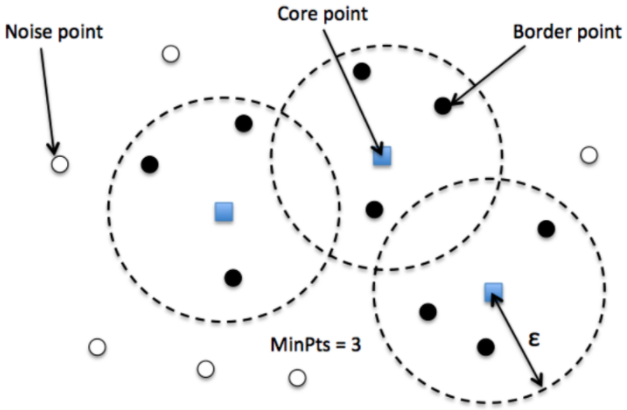
\includegraphics[width=0.6\textwidth]{imagenesResumen/DBSCAN.png}
    \caption{Ejemplo de DBSCAN.}
\end{figure}

\begin{figure}[!htb]
    \centering
    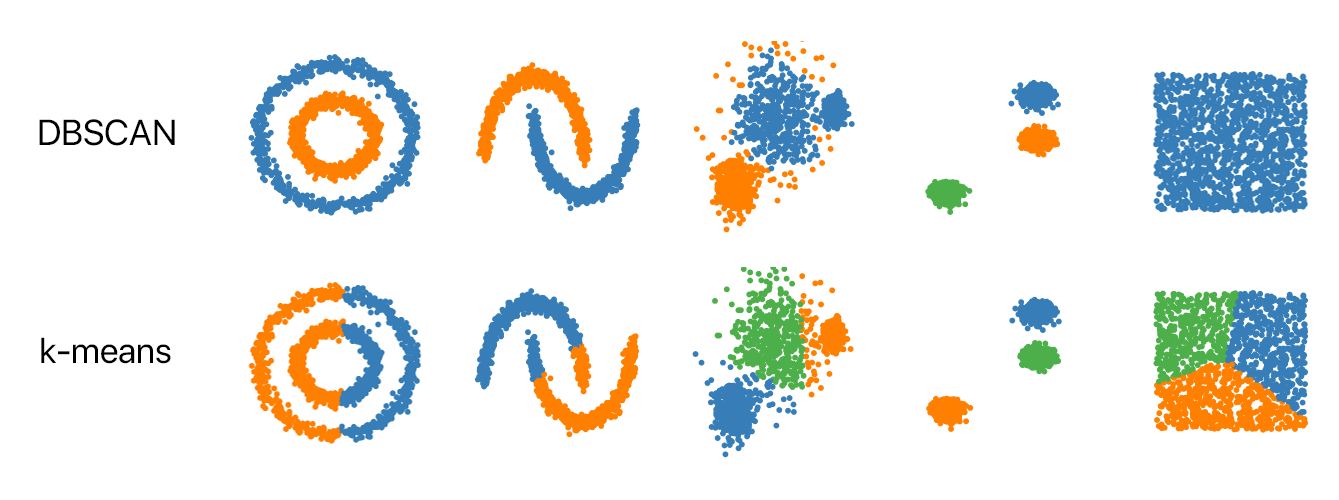
\includegraphics[width=0.9\textwidth]{imagenesResumen/ComparacionKMeansDBSCAN.png}
    \caption{Comparación de la performance de DBSCAN con K-Means.}
\end{figure}

\subsubsection*{Algoritmo}
\begin{enumerate}
    \item Etiquetar cada punto como core, border o noise.
    \item Eliminar los puntos noise.
    \item Poner una arista entre los puntos que son vecinos entre si.
    \item Los componenetes conexas son un cluster.
    \item Asignar los puntos border.
\end{enumerate}


\subsection{HDBSCAN}
Hereda del anterior. Es una mejora. Tiene un valor $\epsilon$ variable, densidad variable para evitar puntos que sean ruido, y mejora la velocidad.

\subsection{Evaluación de clusters}

\subsubsection{Matriz de similitud}

\begin{itemize}
    \item Cuadrada y simétrica.
    \item Similitud entre cada par de instancias.
    \item El resultado es bueno si la matriz es diagonal en bloques.
    \item \textbf{Cohesión} Mide cuan relacionados están los elementos de un cluster
    \item \textbf{Separación} Cuan lejos están los distintos clusters entre si.
\end{itemize}

\begin{figure}[!htb]
    \centering
    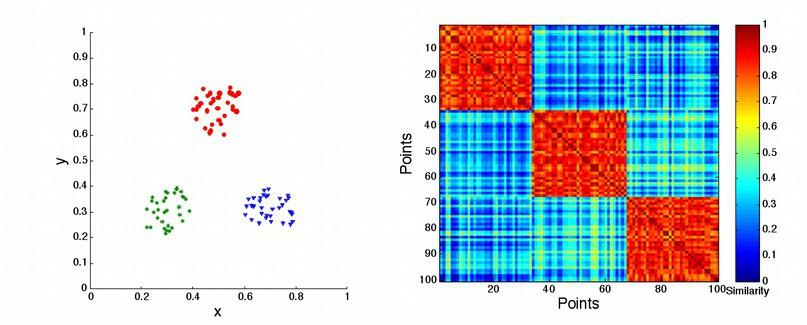
\includegraphics[width=0.7\textwidth]{imagenesResumen/MatrizSimilitud.jpg}
    \caption{A la derecha se puede ver la matriz de similitud. Notar que es diagonal en bloques y los clusters estan bien clasificados.}
\end{figure}

\subsubsection{Coheficiente de Silhouette}
Mientras mas cercano al centro, mas cercano a 1. Se mueve de -1 a 1. Indica que tan bien definidos están los clusters.

\begin{equation}
    s_i = \frac{b_i - a_i}{max\{b_i,a_i\}}
\end{equation}

Siendo $a$ la distancia promedio de $x_i$ hacia otros puntos del mismo cluster, y $b$ siendo la distancia promedio de $x_i$ hacia los puntos del cluster mas cercano.

\begin{figure}[!htb]
    \centering
    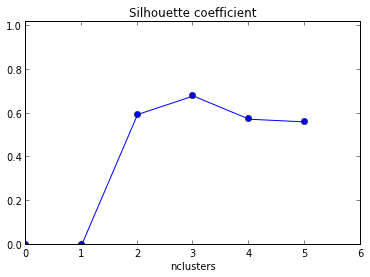
\includegraphics[width=0.5\textwidth]{imagenesResumen/SilhouetteCoef.png}
    \caption{Grafico mostrando el avance con este coeficiente}
\end{figure}

\newpage

\subsubsection{Rand Index}

Mide la similitud entre 2 resultados de clustering. Va de 0 a 1.

\begin{itemize}
    \item a: son los pares que están en un mismo cluster en X y en un mismo cluster en Y.
    \item b: pares que están en distintos clusters en X y en distintos Y.
    \item c: pares que están en un mismo cluster en X, pero en distintos en Y.
    \item d: pares que están en distintos clusters en X y en el mismo en Y.
\end{itemize}

\begin{equation}
    R = \frac{a+b}{a+b+c+d}
\end{equation}

\subsection{Elbow Method}
Método para encontrar el numero ideal de clusters. Se van graficando los resultados a medida que aumenta el K. Se termina eligiendo el numero a partir del cual no hay mejora.

\begin{figure}[!htb]
    \centering
    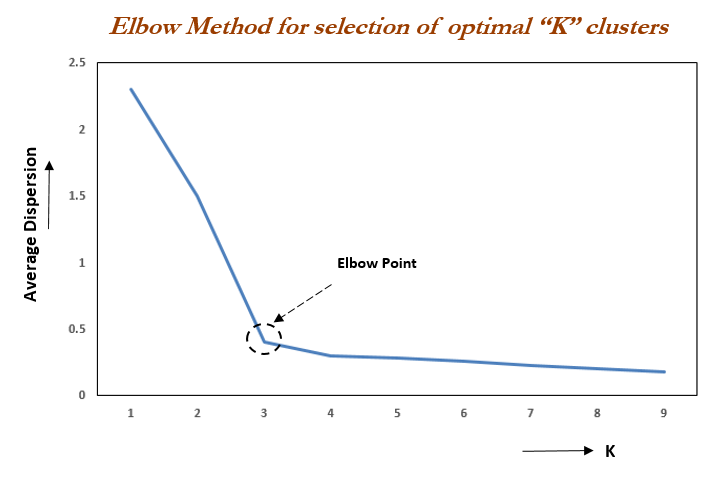
\includegraphics[width=0.8\textwidth]{imagenesResumen/ElbowMethod.png}
    \caption{Método de Elbow. Se puede ver como a partir de 3 no hay una gran mejora.}
\end{figure}

\newpage

\section{Reducciones dimensionales}

Son técnicas que sirven para cuando tenemos una alta dimensionalidad de los datos. Con ellas buscamos proyectar esos datos en un espacio de dimensión menor sin perder información. 

Algunas reducciones posibles son:
\begin{itemize}
    \item Seleccionando variables
    \item Transformando variables
\end{itemize}

\subsubsection*{¿Por que hacerlo?}

\begin{itemize}
    \item Sirve para visualizar mejor el espacio
    \item Puede ayudar a reducir el ruido
    \item Regulariza los datos
    \item Comprime la información
    \item Reduce el computo de los modelos
\end{itemize}

\subsection{PCA}

Dada una variable \begin{math} X = (x_1,...,x_n) \end{math}, buscamos un conjunto de proyecciones lineales ortogonales de \textit{X}, donde las proyecciones estén ordenadas de forma decreciente según su varianza.

\subsubsection*{Notas}
\begin{itemize}

\item La varianza es una medida que cuantifica la cantidad de información que se tiene.

\item El resultado provoca una rotación o cambio del sistema de coordenadas.

\item El método busca rotar el dataset de manera de maximizar la varianza de los datos en proyecciones ortogonales. Para esto asume que los datos se encuentran en un subespacio lineal de dimensión menor a la original.

\item La dirección en que se maximiza es en la del autovector $\mu$ de $\sum$ (matriz de covarianza de los datos) cuyo autovalor $\lambda$ asociado es mayor.

\item La reducción PCA es única. Da siempre el mismo resultado. (Determinista)

\item La proyección de X en $k$ dimensiones esta dado en la matriz $Z = X * V$. Su reconstrucción es con $X = Z * V^{t}$

\item Si la varianza en V es menor a 1, se perdieron datos y la reconstrucción no sera perfecta.

\item \textit{Si todos los valores son iguales, (Var = 0) esa columna no aporta mucho}

\end{itemize}

\subsubsection*{Fortalezas}
\begin{itemize}
    \item No tiene hiperparámetros
    \item No tiene iteraciones
    \item Sin óptimos locales.
\end{itemize}

\subsubsection*{Debilidades}
\begin{itemize}
    \item Limitado a proyecciones lineales.
\end{itemize}

\begin{figure}[!htb]
    \centering
    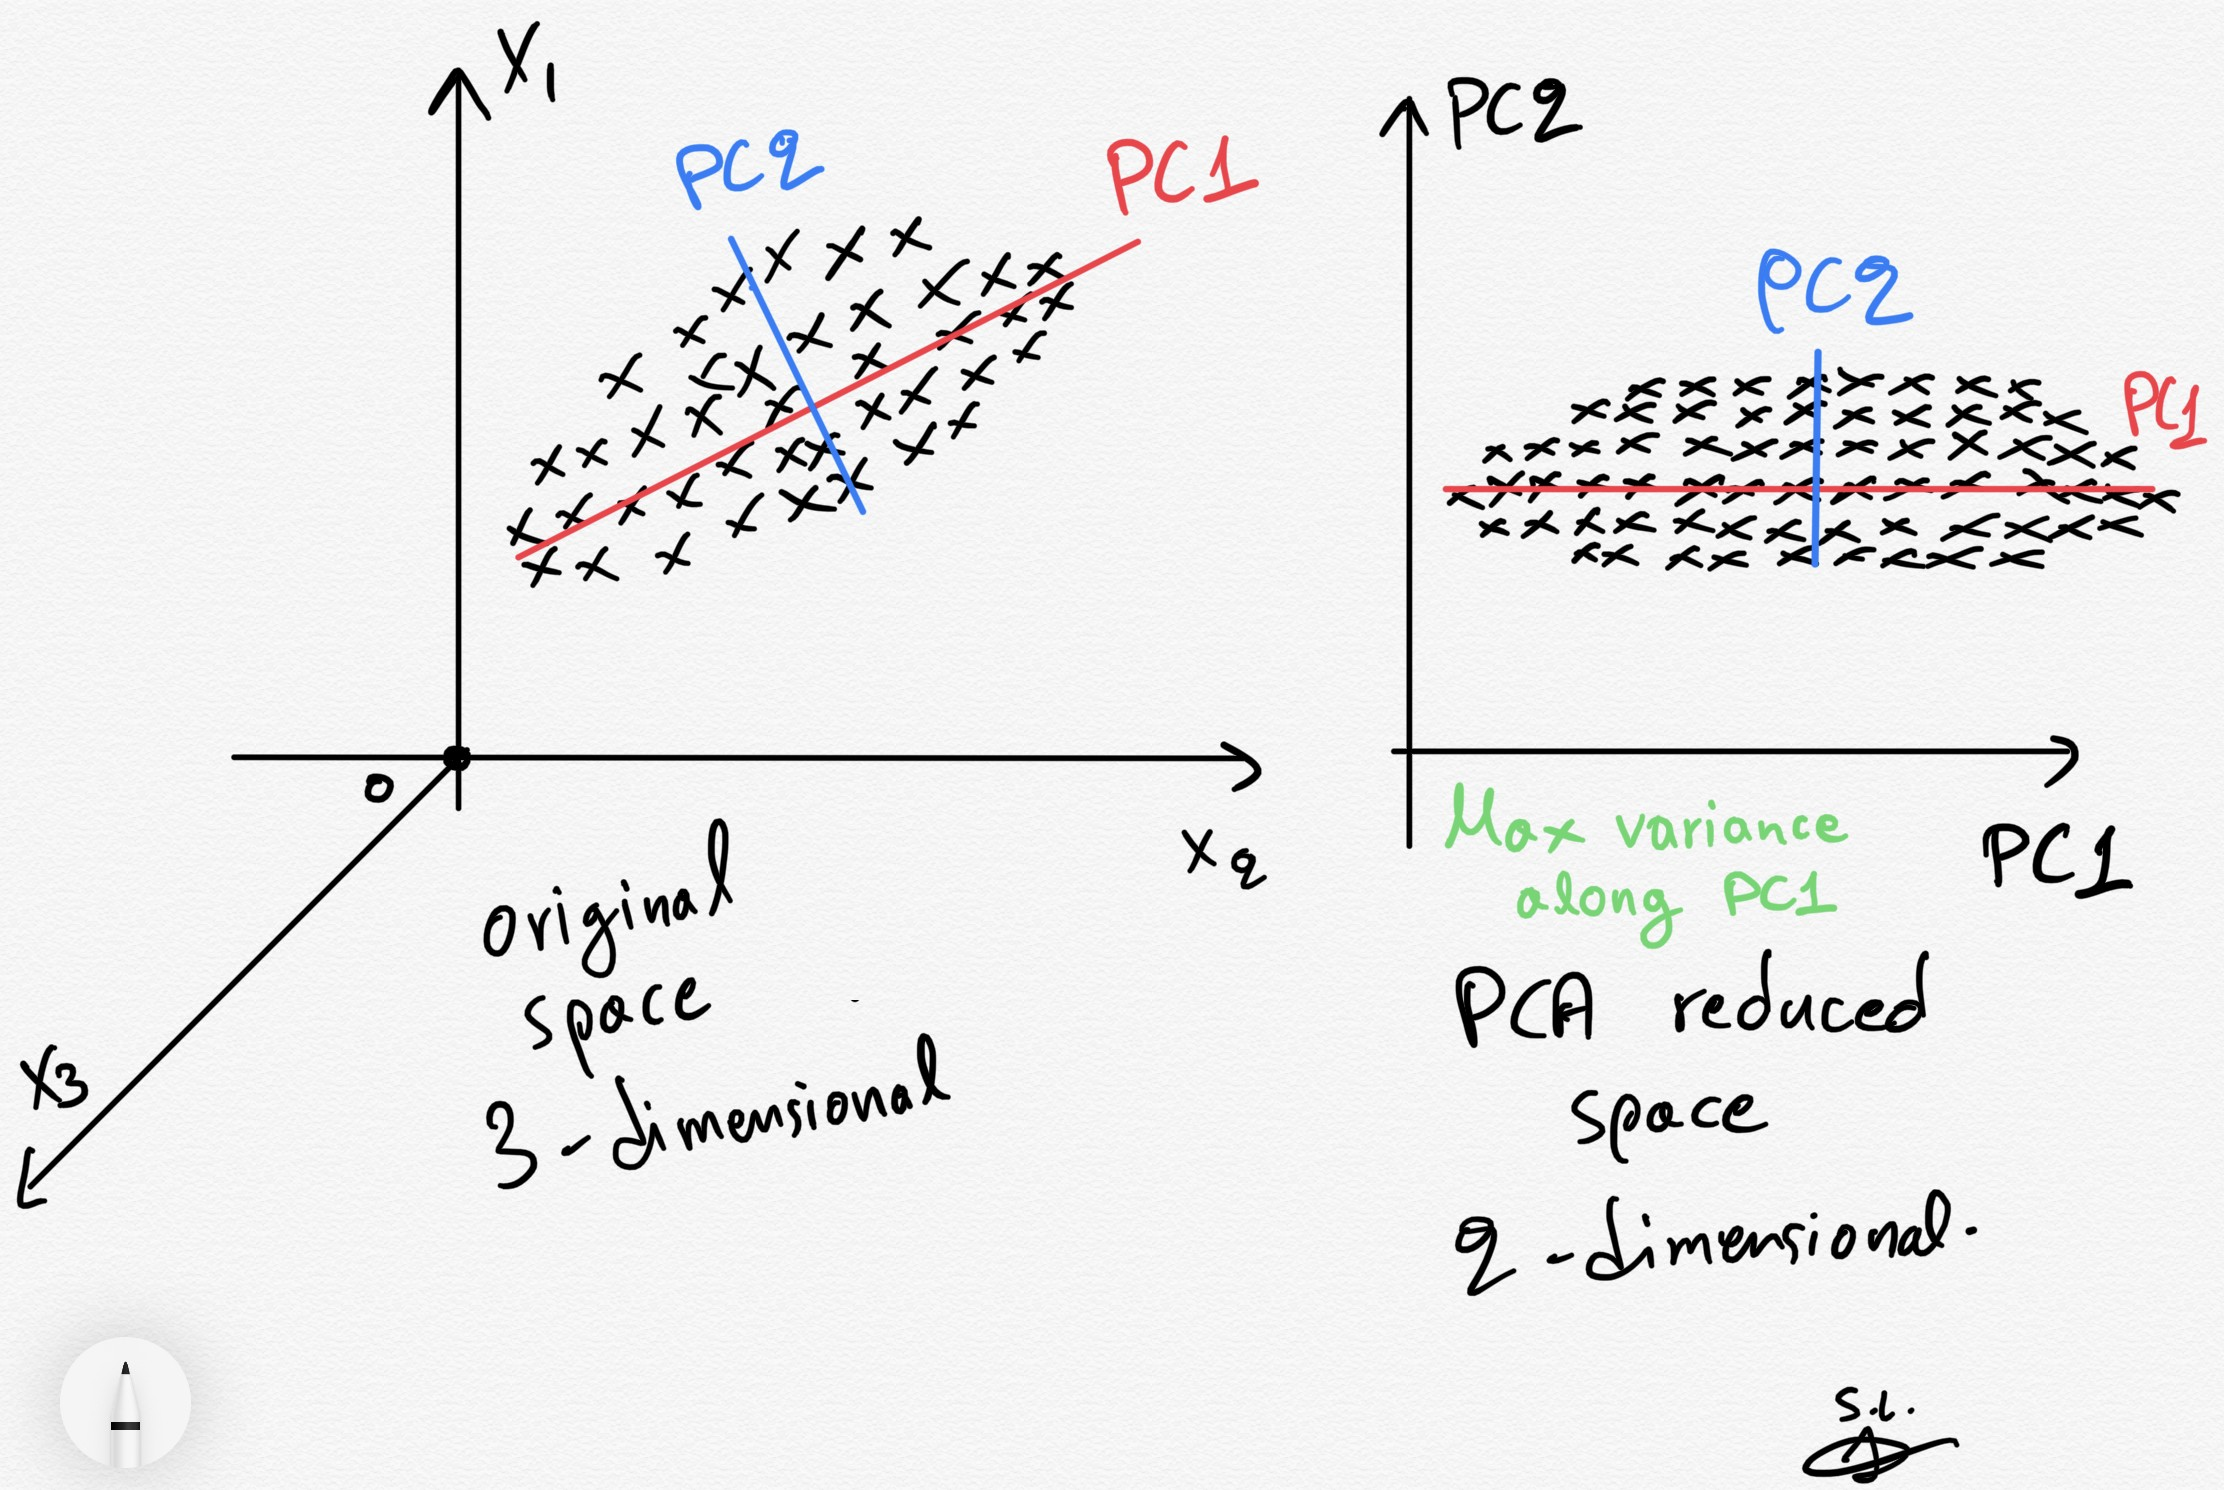
\includegraphics[width=0.9\textwidth]{imagenesResumen/PCA.jpeg}
    \caption{Conversión utilizando PCA}
\end{figure}

Gif mostrando la conversión \href{https://miro.medium.com/max/1556/1*T7CqlFV5aRm6MxO5nJt7Qw.gif}{aquí}.

\subsection{MDS}

Es un método que consiste en preservar la distancia entre los puntos. Intenta ubicarlos en una dimensión menor tal que la distancia se parezca lo mas posible.

\subsubsection*{Fortalezas}
\begin{itemize}
    \item Soporta varios tipos de distancia.
    \item Permite transformaciones no lineales.
\end{itemize}

\subsubsection*{Debilidades}
\begin{itemize}
    \item Optimización iterativa con mínimos locales.
    \item Difícil determinar que distancia usar.
\end{itemize}

\begin{figure}[!htb]
    \centering
    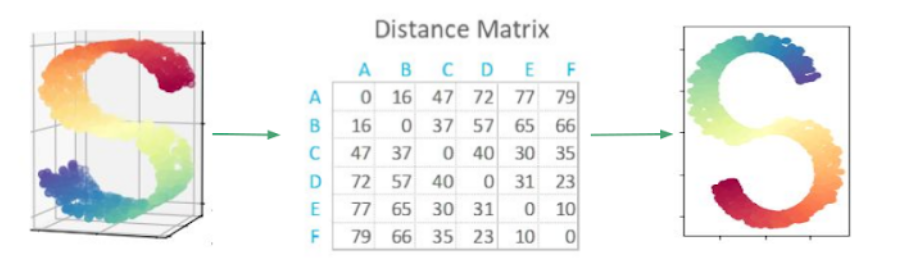
\includegraphics[width=0.9\textwidth]{imagenesResumen/MDS.PNG}
    \caption{Conversión utilizando MDS}
\end{figure}


\subsection{ISOMAP}

Similar al anterior en cuanto a preservar la distancia. Se diferencia en que este busca preservar la geométrica utilizando distancia geodésica.

\subsubsection*{Algoritmo}
\begin{enumerate}
    \item Determinar vecinos mas cercanos.
    \item Construir grafo de vecinos.
    \item Computar el camino mínimo \textit{Ej. Dijsktra}.
    \item Generar matriz de distancias en base al anterior punto, y aplicar MDS.
\end{enumerate}

\subsubsection*{Fortalezas}
\begin{itemize}
    \item Mantiene la estructura.
    \item Permite transformaciones no lineales.
\end{itemize}

\subsubsection*{Debilidades}
\begin{itemize}
    \item Determinar un k de vecinos.
    \item Sensible a ruido.
    \item Muchos vecinos puede hacer que se rompa la distancia geodésica y de algo mas como MDS.
\end{itemize}

\begin{figure}[!htb]
    \centering
    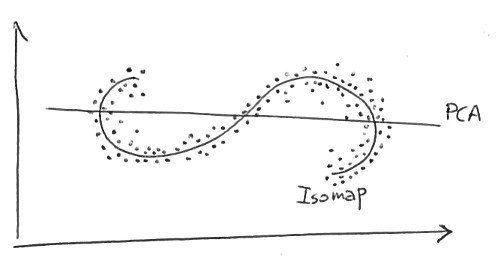
\includegraphics[width=0.7\textwidth]{imagenesResumen/ISOMAP.jpeg}
    \caption{Conversión utilizando ISOMAP.}
\end{figure}

\newpage

\subsection{t-SNE}

La idea detrás de este método es ir de $\mathbb{R}^{n} \Rightarrow \mathbb{R}^{2}$ respetando lo mejor posible los puntos de $\mathbb{R}^{n}$. \textit{Ej. Conservar los grupos como estaban.}

\subsubsection*{Notas}
\begin{itemize}
    \item Se usan las distancias para construir una matriz de probabilidad de ser vecino. mientras mas grande, mas probable es que se este cerca.

    \item Tiene un parámetro, \textit{perplexity}, que mientras mas grande mas vecino se es.
    
    \item Se utiliza el descenso del gradiente.
    
    \item No tiene sentido en \textit{Machine Learning}.
\end{itemize}

\subsubsection*{Algoritmo}
\begin{enumerate}
    \item Iniciar los puntos al azar.
    \item Matriz de probabilidad en X, Y.
    \item Movemos los puntos de Y hasta que se parezcan lo mas posible.
\end{enumerate}

\subsubsection*{Fortalezas}
\begin{itemize}
    \item Muy bueno para visualizar datos.
    \item Conserva estructuras no lineales.
\end{itemize}

\subsubsection*{Debilidades}
\begin{itemize}
    \item Es estocástico (al azar).
    \item Escala en tiempo con dimensiones y puntos.
    \item No sirve para nuevos puntos
\end{itemize}

\newpage

\section{Aprendizaje supervisado}
\subsection{Arboles de decisión}
\begin{itemize}
    \item Sencillo y fácil de comprender.
    \item Sirven como \textit{baseline} trivial.
    \item Sirven como ejemplo para entender la estructura y funcionamiento de otros algoritmos.
    \item Cada nodo evalúa un atributo.
    \item El nodo tiene tantos hijos como posibles atributos tenga.
    \item Si las instancias están lo suficientemente bien clasificadas termino (Se vuelven hojas).
\end{itemize}

\subsubsection*{¿Cual es el mejor atributo?}
Lo podemos medir con distintos indicadores.
\begin{itemize}
    \item \textbf{Pureza de Gini} Se elige el que mas reduce la impureza. 
    
    \begin{math}
    Gini(S) = 1 - \sum_{c\in Clases}(\frac{|S_c|}{|S|})^2
    \end{math}
    
    Siendo $S_c$ las instancias de la clase $c$.
    
    \begin{math}
    GiniGain(S,A) = Gini(S) - \sum_{v\in Valores(A)}\frac{|S_v|}{|S|} \cdot Gini(S_v)
    \end{math}
    
    
    \item \textbf{Ganancia de información} Se busca maximizar la ganancia. 
    
    Entropía de una muestra:
    \begin{math}
    H(S) = \sum_{c\in Clases} - p_c \cdot log_2 p_c
    \end{math}
    
    Siendo $p_c$ la proporción de instancias S pertenecientes a C.
    
    \begin{math}
    InfoGain(S,A) = H(S) - \sum_{v\in Valores(A)} \frac{|S_v|}{|S|} H(S_v)
    \end{math}
    
\end{itemize}

Ambos criterios son numéricamente similares.


\subsubsection*{Fortalezas}

\begin{itemize}
    \item Interpretabilidad
    \item Similar a como decide el humano
    \item Acepta varios tipos de input
    \item Maneja bien  los missing values
\end{itemize}

\subsubsection*{Debilidades}

\begin{itemize}
    \item Llegan a menos precisión
    \item Varianza alta
\end{itemize}

\subsubsection*{Overfitting}

Sucede cuando se 'aprendió de memoria' los datos. En el caso de los arboles se puede ver cuando estos se vuelven muy profundos, esto puede llegar al caso de que en cada hoja haya incluso un solo dato. Como consecuencia de esto, el modelo generalizaría mal.

Las soluciones en arboles son, parar a partir de cierta profundidad, o realizar una poda (Pruning)  (sacar ramas cuando mejore la performance). Otra opción es Post-Pruning.

\newpage

\subsection{KNN}
Este modelo busca predecir la instancia de un nuevo punto a partir de sus vecinos.

\begin{itemize}
    \item Mientras mas cerca a un punto, mas peso deben de tener. Ponderar sobre la distancia.
    \item Si se toman Ks mas grandes, se empieza a suavizar la variación.
    \item Se rompe mientras mas dimensionalidad se tenga.
    \item Es un modelo simple.
    \item El entrenamiento es muy rápido, ya que consiste en agarrar los puntos y ver solamente.
    \item La contraparte es que la consulta se vuelve lenta.
    \item También como funciona el modelo hace que se ocupe mucho espacio en disco.
    \item Es susceptible a escalas.
\end{itemize}

\begin{figure}[!htb]
    \centering
    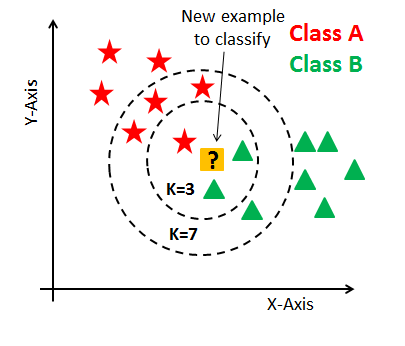
\includegraphics[width=0.5\textwidth]{imagenesResumen/KNN.png}
    \caption{Ejemplo de KNN.}
\end{figure}


\subsection{Naive Bayes}
Este es un modelo que se basa en el calculo de probabilidades utilizando la teoría de probabilidad bayesiana. Asume que todos los sucesos son independientes para hacerlo.

\begin{itemize}
    \item Cuenta la cantidad de veces que aparece cierta característica básicamente.
    \item Tiene de hiper-parámetro el smoothing (suavizado) que evita que haya casos con probabilidad 0.
    \item No tiene en cuenta el orden. Si se quiere, se pueden utilizar n-gramas.
    
\end{itemize}

%quizas meter algun ejemplo?
\newpage

\subsection{SVM}

Modelo que busca que una recta/hiper-plano separe las clases de la mejor forma posible. Busca esto sin tener que modelar la distribución de los datos de cada clase.

\begin{itemize}
    \item Es iterativo, puede escalar en tiempo.
    \item Va a converger, no hay óptimos locales.
    \item Las instancias mas cercanas se vuelven 'Support Vectors'
    \item Busca maximizar el M (margen), el espacio entre los distintos tipos de puntos.
    \item Si no encontró una recta/hiper-plano, los puntos no son linealmente separables.
    \item Se consigue la recta creando una nueva dimensión. Como esto es costoso se puede utilizar Kernel Trick, que hace que se 'piense que esta en otra dimensión'. \textit{Ej. lineal, polinomial, sigmoideo, rbf}
\end{itemize}

\begin{center}
\begin{math}
W \cdot X + b > 0
\end{math}
Para la clase A.

\begin{math}
W \cdot X + b < 0
\end{math}
Para la clase B.
\end{center}

\subsubsection*{Hard Margin vs Soft Margin}

En Hard Margin los puntos están perfectamente separados. Esto hace que el modelo no funciones con outliers y ruido.

En Soft Margin se permite algo de ruido y outliers.

Este hiper-parámetro se controla con el C. A mayor C se tiene HM, a menor SM.

\begin{figure}[!htb]
    \centering
    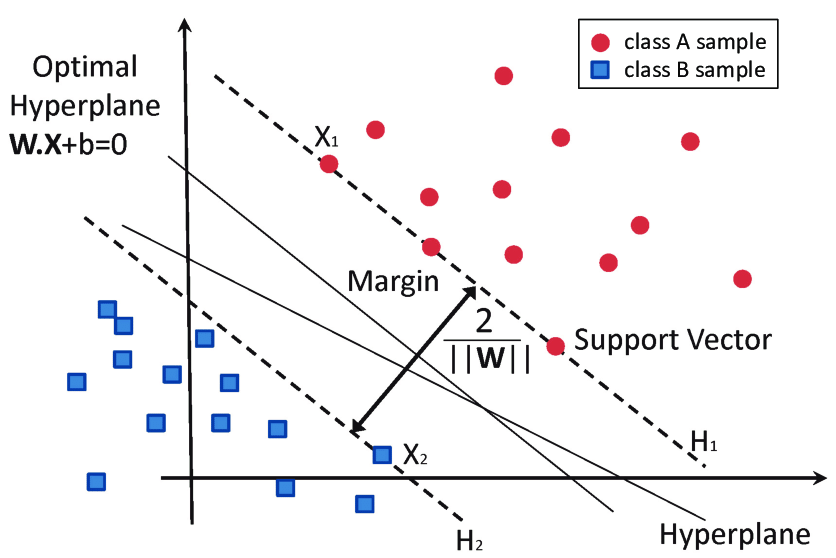
\includegraphics[width=0.7\textwidth]{imagenesResumen/SVM.png}
    \caption{Ejemplo de SVM.}
\end{figure}

\newpage

\section{Evaluación y selección}

La idea es evaluar sobre datos que no se hayan usado en el entrenamiento. Para ello, nos guardamos una parte de los mismos para usarlos mas adelante. (10\% a 25\%)

También se cuenta con una parte que se conoce como holdout, que es para evaluar cuando el modelo esta por salir a producción.

Algo a tener en cuenta, es evitar los \textit{data leaks}, esto sucede cuando parte de lo que tenes en tu parte de entrenamiento aparece en la de evaluación.

\subsection{¿Como hacer el particionado?}

El particionado tiene que ser random. No debe de agarrar las primeras x instancias y listo. Se le puede pedir cuando se esta partiendo que respete la distribución de las clases. Muy útil para cuando se tienen casos muy des-balanceados. \textit{Ej. Clase positivo es el 10\% y el resto negativo.}

\begin{figure}[!htb]
    \centering
    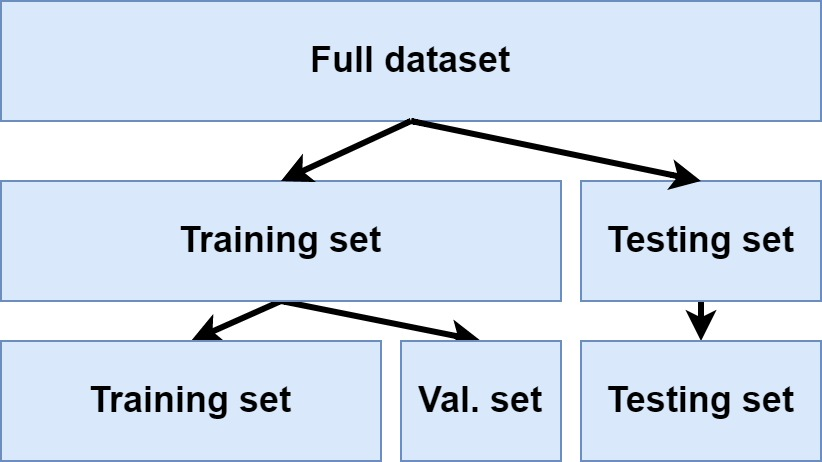
\includegraphics[width=0.6\textwidth]{imagenesResumen/TrainTestSplit.jpg}
    \caption{Division de los datos}
\end{figure}

\subsection{Crossvalidation K-Fold}

Consiste en dividir varias veces los datos, e ir cambiando el conjunto. Esto hace que se disminuya el riesgo de tener una mala partición.

\subsubsection*{Algoritmo}
\begin{enumerate}
    \item Desordenar los datos
    \item Separar en k folds del mismo tamaño
    \item De $i = 1,..k$, entrenar con todos menos $i$. Después evaluar con $i$  
\end{enumerate}

\textit{Nota: Stratified K-fold mantiene las proporciones.}

\begin{figure}[!htb]
    \centering
    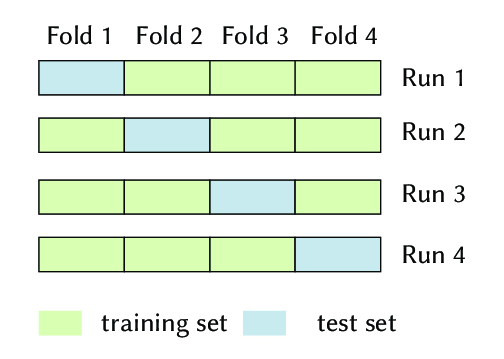
\includegraphics[width=0.6\textwidth]{imagenesResumen/CVKFold.png}
    \caption{Funcionamiento de CV K-fold}
\end{figure}


\newpage

\subsection{Grid Search}

Es un método con el cual se buscan los mejores hiper-parámetros de cada modelo. Escala mucho en tiempo si no se paraleliza, esto se debe a que el algoritmo consiste en ir agregando \textit{for} por cada hiper-parámetro. Una alternativa es ir eligiendo aleatoriamente (Random Search).

\begin{minted}{python}
best_score = None
best_hiperparams = None
for h1 in valores_hiperparametro_1:
    for h2 in valores_hiperparametro_2:
          ...
          for hn in valores_hiperparametro_n:
              kf = StratifiedKFold(n_splits=5)
              metrics = []
              for fold_idx, (train_index, test_index) in enumerate(kf.split(X, y)):
                  clf = Clasificador(h1, h2, ..., hn)
                  clf.fit(X[train_index], y[train_index])
                  metrics.append(metric(y[test_index], clf.predict(X[test_index])))
              if not best_score or np.mean(metrics) < best_score:
                  best_score = np.mean(metrics)
                  best_hiperparams = [h1, h2, ..., hn]
\end{minted}
\begin{center}
   \textit{Código genérico de grid search en Python.}
\end{center}





\subsection{Métricas}
\begin{itemize}
    \item Accuracy: Evalúa directamente a cuantos le pegamos.
    \item Matriz de confusión: Ver imagen \ref{MatrizDeConfusion}
    \item Precision: No le interesa si perdemos alguno, quiere saber a cuantos le pegamos de los que decimos que son. 
    \item Recall: Nos importa la mayor cantidad de casos que predecimos reales.
    \item F1-Score: Permite tener un único numero para evaluar un modelo.
    \item Curva ROC: Es un gráfico que me dice de forma visual que tan buen modelo tengo. Ver imagen \ref{ROCCurve}
    \item AUC-ROC: Valor que surge de medir el área bajo la curva ROC.
    \item Hay otros como True Positivity Rate o el True Negative Rate.
\end{itemize}

\begin{equation}
    Precision = \frac{TP}{TP+FP}
\end{equation}


\begin{equation}
    Recall = \frac{TP}{TP+FN}
\end{equation}

\begin{equation}
    F1-Score = 2 \cdot \frac{Precision \cdot Recall}{Precision + Recall}
\end{equation}

\begin{figure}[!htb]
    \centering
    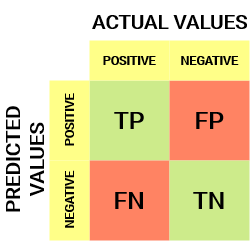
\includegraphics[width=0.5\textwidth]{imagenesResumen/MatrizDeConfusion.png}
    \caption{Matriz de confusión}
    \label{MatrizDeConfusion}
\end{figure}

\begin{figure}[!htb]
    \centering
    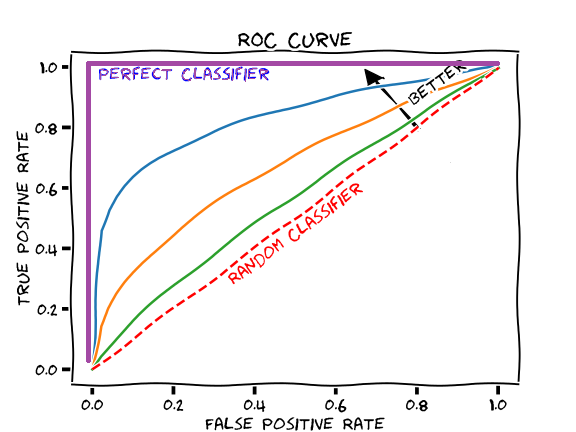
\includegraphics[width=0.7\textwidth]{imagenesResumen/ROCCurve.png}
    \caption{Gráfico mostrando posibles casos de ROC Curve}
    \label{ROCCurve}
\end{figure}



Para encontrar la mejor combinación, hay que explorar el espacio de posibles combinaciones, usando idealmente \textit{K-fold} para medir el desempeño.

\newpage

\section{Ensambles}

Un ensamble es una unión de muchos modelos juntos haciendo predicciones sobre un problema. Cada modelo ajustaría de forma distinta, agarrando una parte del concepto que se busca. Esto causa que se tenga un bajo sesgo y se reduzca la varianza.

\begin{figure}[!htb]
    \centering
    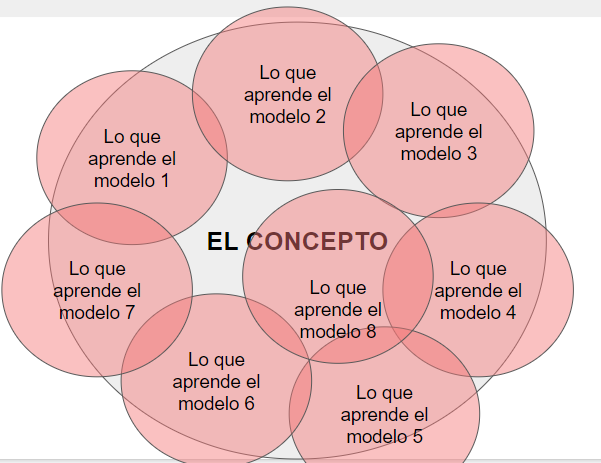
\includegraphics[width=0.6\textwidth]{imagenesResumen/ConceptoEnsamble.PNG}
    \caption{Funcionamiento de los ensambles}
\end{figure}

\subsection{Bagging}

Ensamble que funciona construyendo nuevos conjuntos de entrenamiento usando bootstrap. Realiza un muestreo con remplazo de las instancias.

\begin{figure}[!htb]
    \centering
    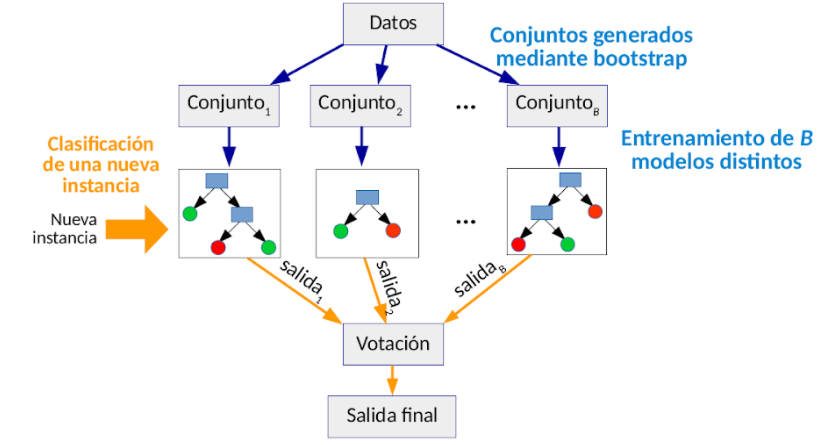
\includegraphics[width=0.7\textwidth]{imagenesResumen/Bagging.PNG}
    \caption{Ej. Bagging}
\end{figure}

La tasa de error reduce con el numero de clasificadores. Mientras mas tenga mas me voy a estar acercando al concepto. No suele aumentar el sobre-ajuste en este caso.

\textit{Problema: Si se utiliza con arboles, y se tienen pocos atributos importantes, los arboles se van a parecer entre si. Por eso conviene Random Forest en ese caso.}

\subsection{Random Forest}

\begin{itemize}
    \item Igual a bagging, pero en cada nodo solo hay un subconjunto de atributos elegidos al azar.
    \item Es bueno para selección de features.
    \item Al aumentar la cantidad de arboles no aumenta el overfitting.
\end{itemize}

\begin{figure}[!htb]
    \centering
    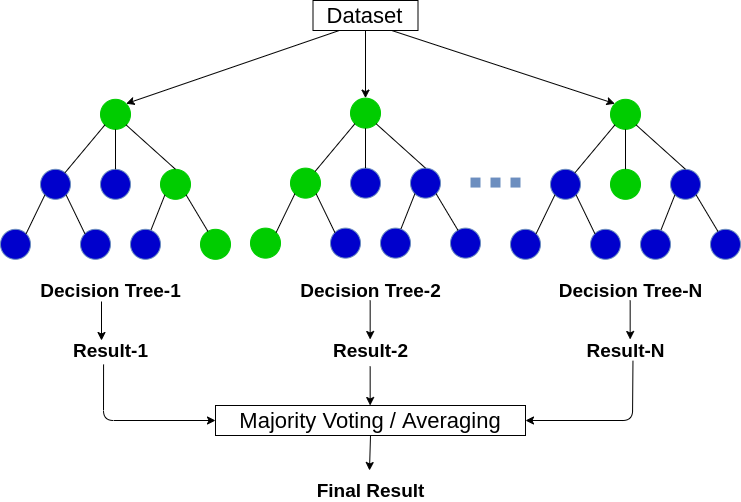
\includegraphics[width=0.7\textwidth]{imagenesResumen/RandomForest.png}
    \caption{Forma de Random Forest}
\end{figure}


\subsection{Boosting}
\begin{itemize}
    \item El sesgo baja en este caso, cada modelo mira mas los datos.
    \item Se comienza con un modelo simple entrenado sobre todos los datos.
    \item En cada iteración se entrena dando mayor importancia a los datos mal clasificados por las iteraciones anteriores.
    \item Puede sobre ajustar.
    \item Algunas implementaciones son AdaBoost, GradientBoost, XGBoost.
\end{itemize}

\begin{figure}[!htb]
    \centering
    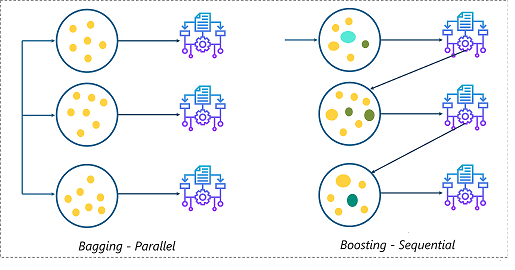
\includegraphics[width=0.7\textwidth]{imagenesResumen/Boosting.png}
    \caption{Comparación Boosting y Bagging}
\end{figure}

\subsection{Híbridos}
\subsubsection{Voting}
Consiste en construir N modelos usando los mismos datos, y luego tomar la predicción mayoritaria.

\begin{figure}[!htb]
    \centering
    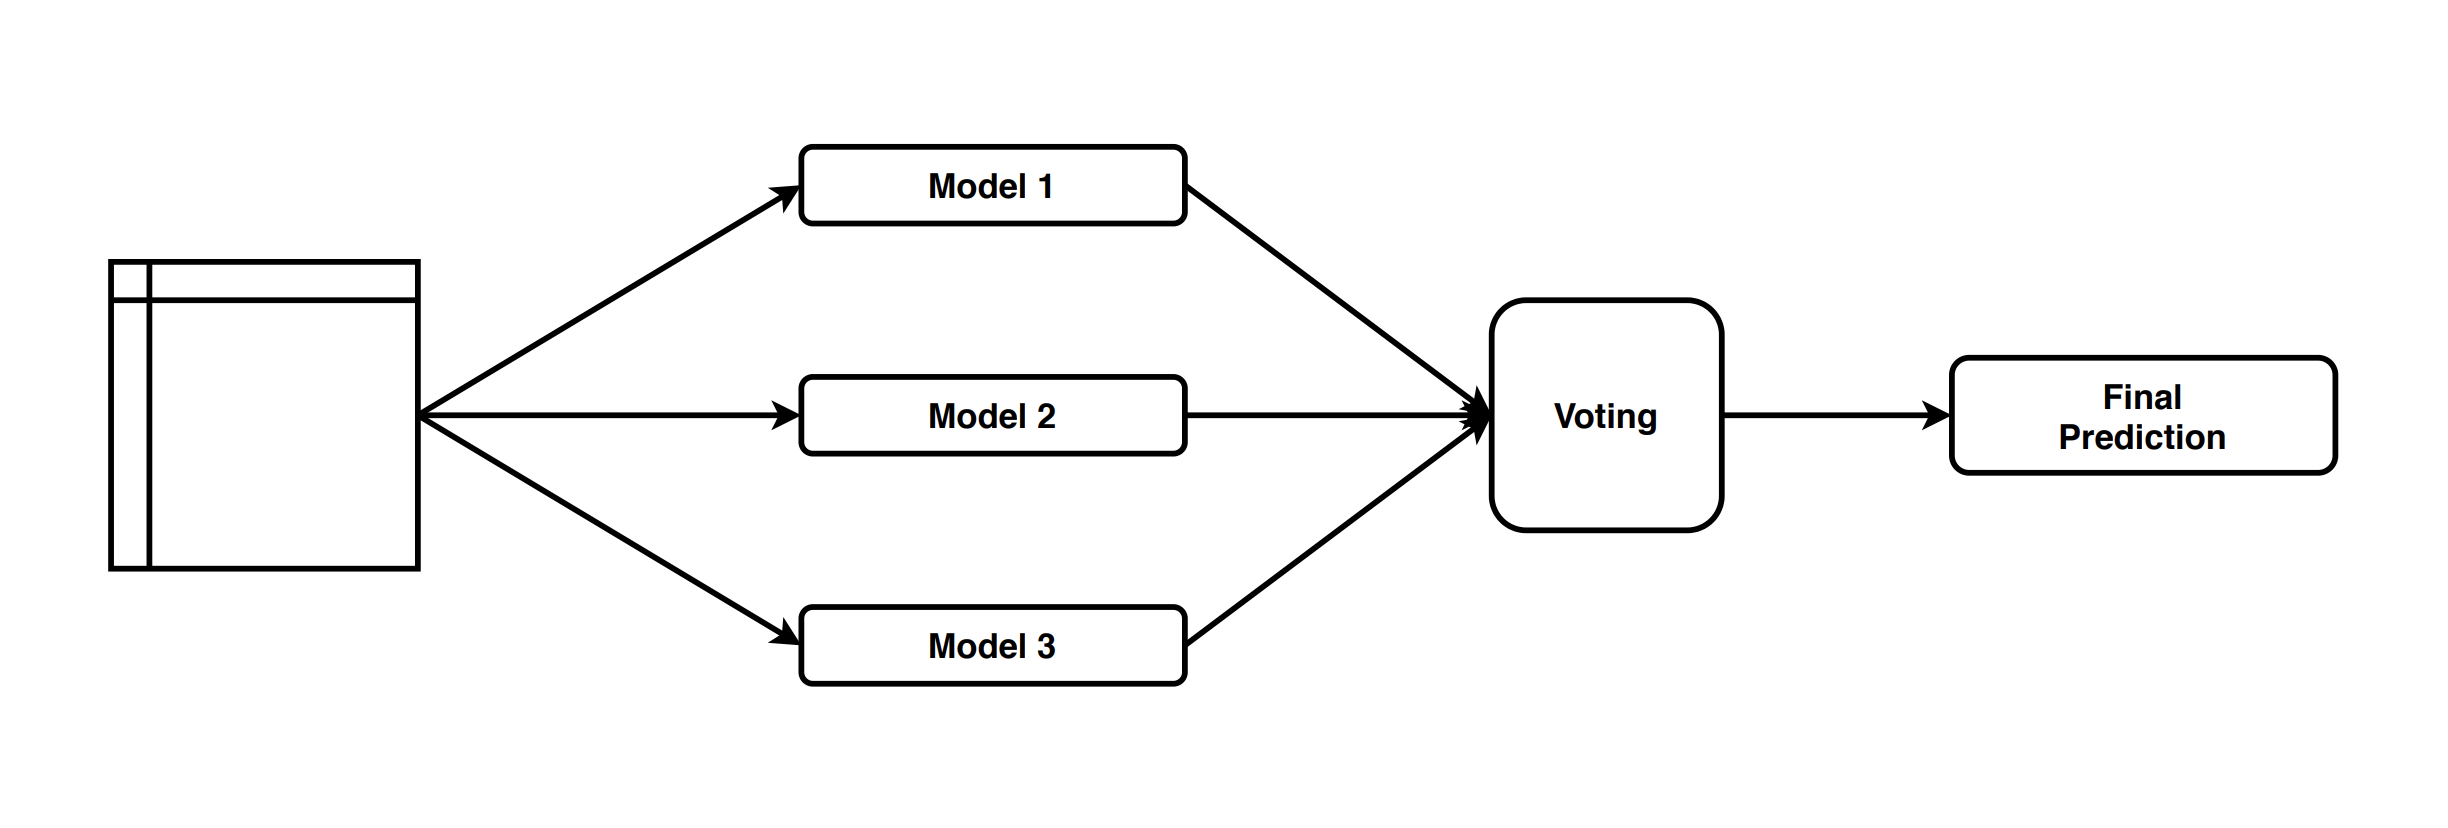
\includegraphics[width=0.8\textwidth]{imagenesResumen/Voting.png}
    \caption{Sistema de Voting}
\end{figure}

\newpage

\subsubsection{Stacking}
Entrenar distintos modelos base, y uno mas que al final recibe las predicciones realizadas. Este ensamble es una mejora del método de votación. Este agregado que remplaza el sistema de votación es de meta-aprendizaje. Generalmente son arboles, NB, SVM, o Perceptron para el modelo final.

\begin{figure}[!htb]
    \centering
    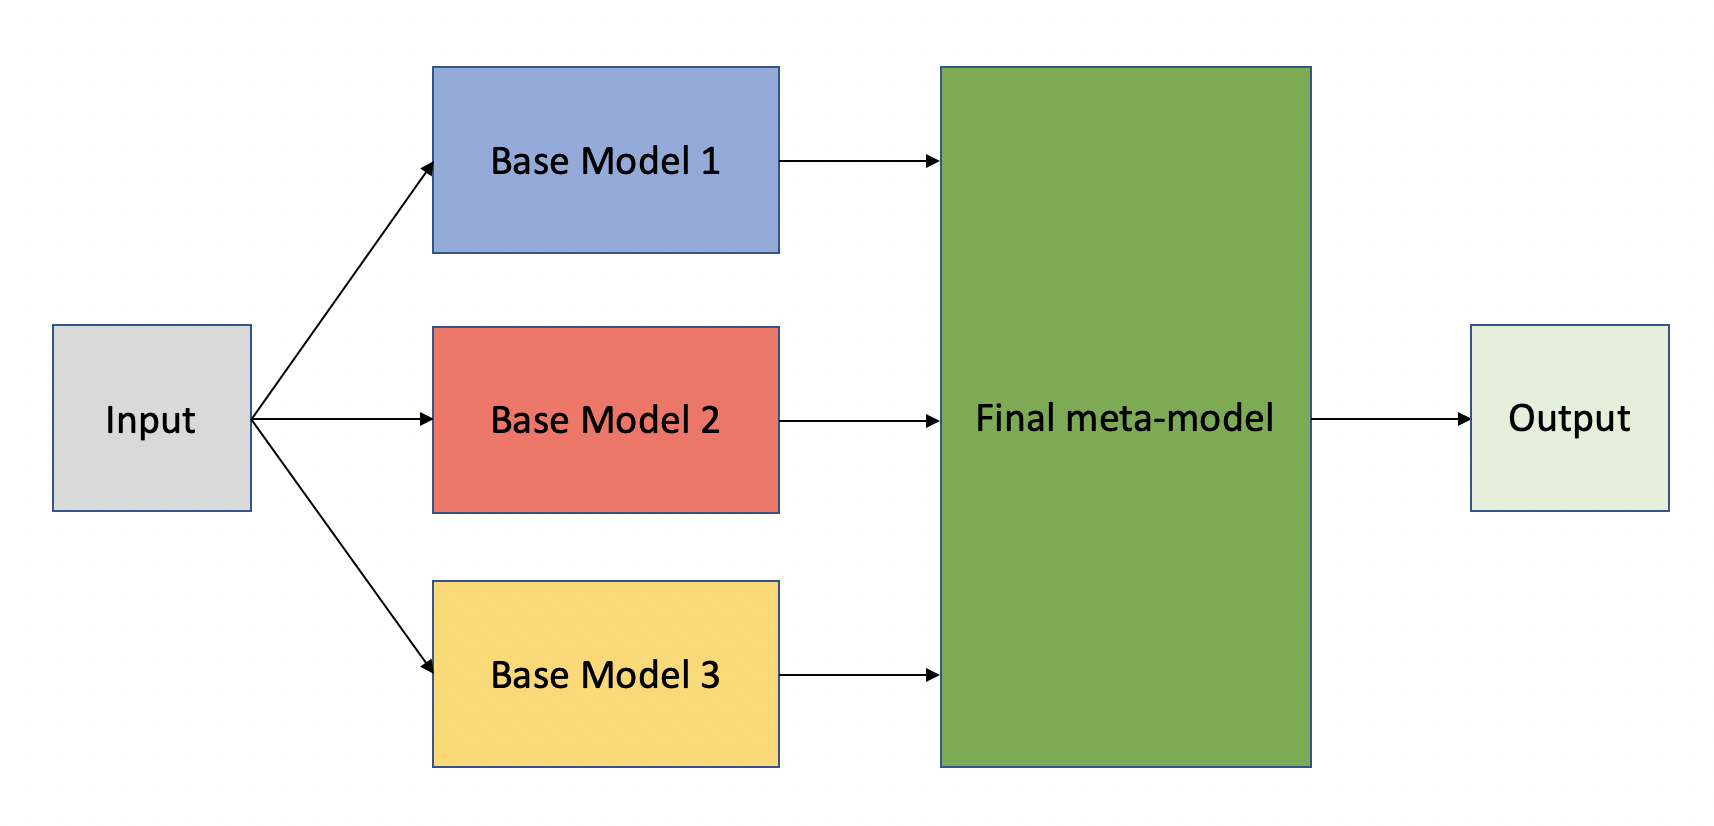
\includegraphics[width=0.8\textwidth]{imagenesResumen/Stacking.png}
    \caption{Sistema de Stacking}
\end{figure}

\subsubsection{Cascading}
En este ensamble se pasan sucesivamente los datos de un modelo a otro. Cada capa tendría un solo modelo, el cual se entrenaría sobre las instancias con baja certeza del modelo anterior. Se suele usar cuando se necesita una alta certeza de la predicción. \textit{Ej. Robo de tarjeta de crédito}


\begin{figure}[!htb]
    \centering
    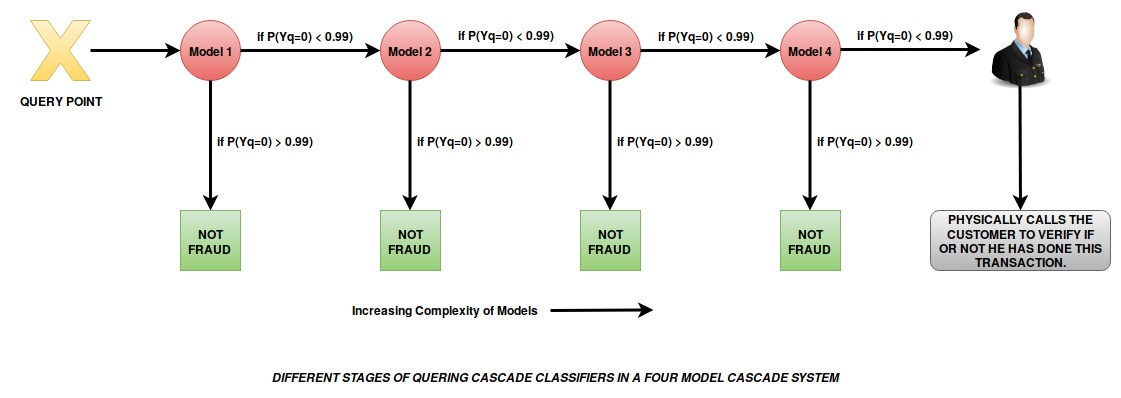
\includegraphics[width=0.9\textwidth]{imagenesResumen/Cascading.jpeg}
    \caption{Ejemplo de Cascading}
\end{figure}


\textit{Nota: Cascadas muy profundas pueden producir overfitting.}

\newpage


\section{Regresiones}

Cada instancia tiene un valor numérico, se quieren predecir una o mas respuestas a partir de varios atributos.  (la funcion es desconocida.)

\begin{equation}
    Y \approx f(X_1, X_2,..., X_n)
\end{equation}


Para evaluarlo tenemos un rango de incerteza.

\subsubsection*{Error cuadrático medio}
\begin{equation}
    MSE = \frac{1}{n} \sum^{n} (y^{i}-\hat{y}^{i})^{2}
\end{equation}

\subsection{Arboles de regresión}
\begin{itemize}
    \item En cada nodo usar reducción del desvío estándar.
    \item Al llegar a una hoja se devuelve el promedio de las Y sobre las instancias que tenga.
\end{itemize}


\subsection{KNN de regresión}
Dada una instancia, se devuelve el promedio ponderado de los valores de sus vecinos. (Z)

\begin{figure}[!htb]
    \centering
    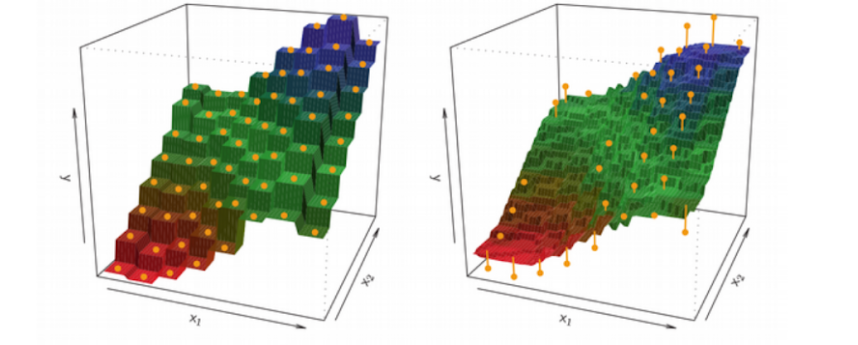
\includegraphics[width=0.9\textwidth]{imagenesResumen/KNNRegresion.PNG}
    \caption{Ejemplo de KNN en regresiones.}
\end{figure}

\subsection{Regresión lineal}
Se supone una relación lineal con una variable y se procede en la cuenta. Cuadrados mínimos es una variante.

\begin{equation}
    y \approx \beta_0 + \beta_1 X_1 + ... + \beta_p X_p
\end{equation}

Para estimar los coeficientes, se igualan a 0 las derivadas. Si algún coeficiente da 0, significa que esa feature no tiene importancia para lo que se quiere predecir.

Si hay error, existe la posibilidad de que sea debido a que la relación no es lineal.

\textbf{Residual Sum of Squares}

\begin{equation}
    RSS = \sum^{n} (y^{i}-\hat{y}^{i})^{2}
\end{equation}


\subsection{Residual Plot}

Forma de observar los residuos que nos da el modelo. Si da algo que no es razonable, dudar de que sea lineal. El gráfico nos tiene que dar una nube de puntos. No se tienen que ver relaciones.

\begin{figure}[!htb]
    \centering
    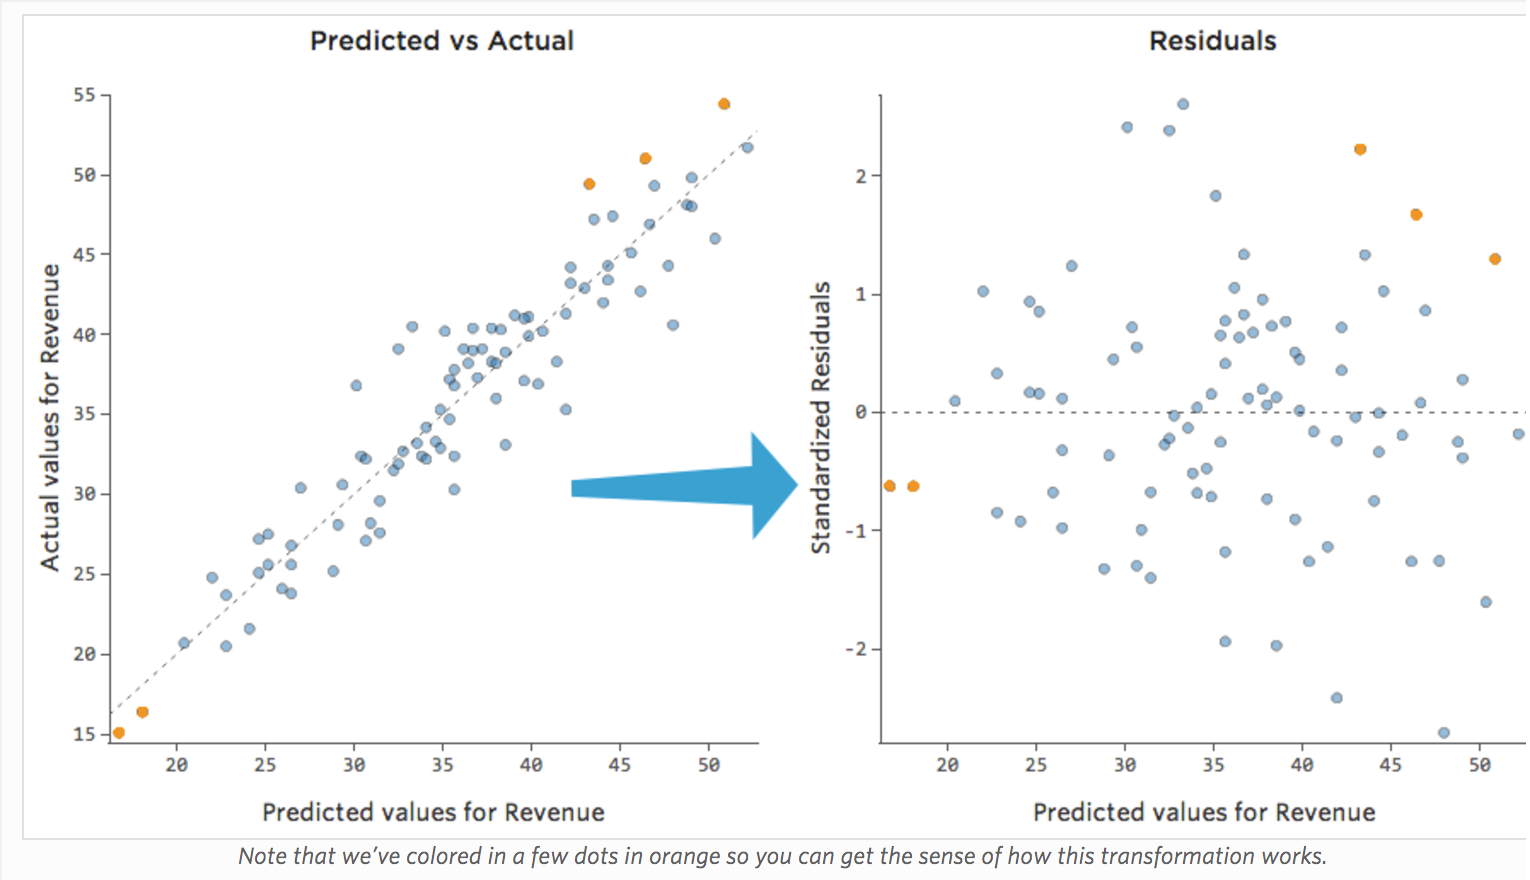
\includegraphics[width=0.9\textwidth]{imagenesResumen/ResidualPlot.png}
    \caption{Ejemplo mostrando un gráfico de residuos. Notar que se ve que es como una nube de puntos. No se nota algún patrón o estructura en particular.}
\end{figure}


\subsection{Regularización} \label{regularizaciones}
\begin{itemize}
    \item Técnica para evitar el overfitting.
    \item Busca hacer mas homogéneos los modelos.
    \item Reduce varianza pero aumenta el sesgo de los estimadores.
    \item Hay que estandarizar las variables.
\end{itemize}

\begin{equation}
    Z = \frac{X_i - \mu}{\sigma}
\end{equation}

\subsubsection*{Causas de overfitting}
\begin{itemize}
    \item Features irrelevantes: No tienen relacion con el target. \textit{Tener cuidado cuando el numero de caracteristicas esta cerca del de observaciones.}
    \item Features correlacionados: El modelo se hace asumiendo independencia.
    \item Coeficientes muy grandes: A mayor valor absoluto, mas puede cambiar la respuesta prevista.
\end{itemize}

Debido a estos problemas, se busca restringir a los coeficientes. Se consigue modificando la función de perdida.

\begin{equation}
    RSS = \sum^{n} (y^{i}-\hat{y}^{i})^{2} + \lambda \sum^{M} |\hat{\beta}_j|^{q}
\end{equation}

\subsubsection{Ridge}
Se tiene cuando q = 2. Hace que el sesgo crezca y la varianza baje a medida que se aumente $\lambda$.

\textbf{Teorema}: Siempre existe un valor de $\lambda$ tal que el MSE de Ridge sea menor que el MSE de mínimos cuadrados.

\subsubsection{Lasso}
Es el caso en que q = 1. Esta regularización puede llegar a anular coeficientes, por lo que puede usarse como selección de variables.

\subsubsection{Elastic Net}
Es una combinación de Lasso y Ridge. Agrega ambos términos a la cuenta, haciendo que cada uno aporte lo valioso que tiene.

\subsection{Robustez}
\subsubsection*{Outlier}
\begin{itemize}
    \item Observación que se desvía tanto de las otras observaciones como para levantar sospechas de que fue generada por otro mecanismo.
    \item En algunos casos nos puede interesar encontrarlo. \textit{Ej. Robo de tarjeta de crédito}
    \item En otros casos es simplemente molesto.
\end{itemize}


Para agregarlo hay que cambiar la función de perdida.

\subsubsection{L1}
Remover el cuadrado y usar directamente el modulo. Lo malo de este caso es que no es bueno para derivarla.

\subsubsection{M estimadores}
\begin{equation}
    \hat{\beta} = arg min_\beta \sum^{n} \rho(\frac{ y_{i}-\beta_0-\sum^{p}\beta_j \cdot X_{ij}}{\hat{\sigma}})
\end{equation}

Para $\rho$ se usan distintas funciones. \textit{Ej. Cuadratica, Huber, Bicuadrada}

Para $\beta$ se deriva nuestra función de perdida y se ve que $\beta$ la igualan a 0.

Esto hace que los outliers tengan poca influencia en el modelo.

%imagen de la recta y de las funciones

\subsubsection{RANSAC}
Forma mas algorítmica. Se seleccionan n valores random, se hace un ajuste de regresión con esos valores, y con esto se evalúa cuales puntos restantes pueden pertenecer con una distancia 'd' (hay que definir también la cantidad mínima de puntos internos para considerarlo un buen modelo). Este algoritmo es iterativo, sirve mucho para cuando hay muchos outliers o ruido.

Gif mostrando el algoritmo en funcionamiento \href{https://upload.wikimedia.org/wikipedia/commons/c/c0/RANSAC_LINIE_Animiert.gif}{aquí}.

\subsubsection{THEIL-SEN}
Otra forma algorítmica. Se toman la mediana de las pendientes calculadas de a pares y me quedo con esa, despues es repetir de forma similar para la ordenada al origen. Es 'insensitivo' a outliers. No depende de hiper-parámetros.

\begin{figure}[!htb]
    \centering
    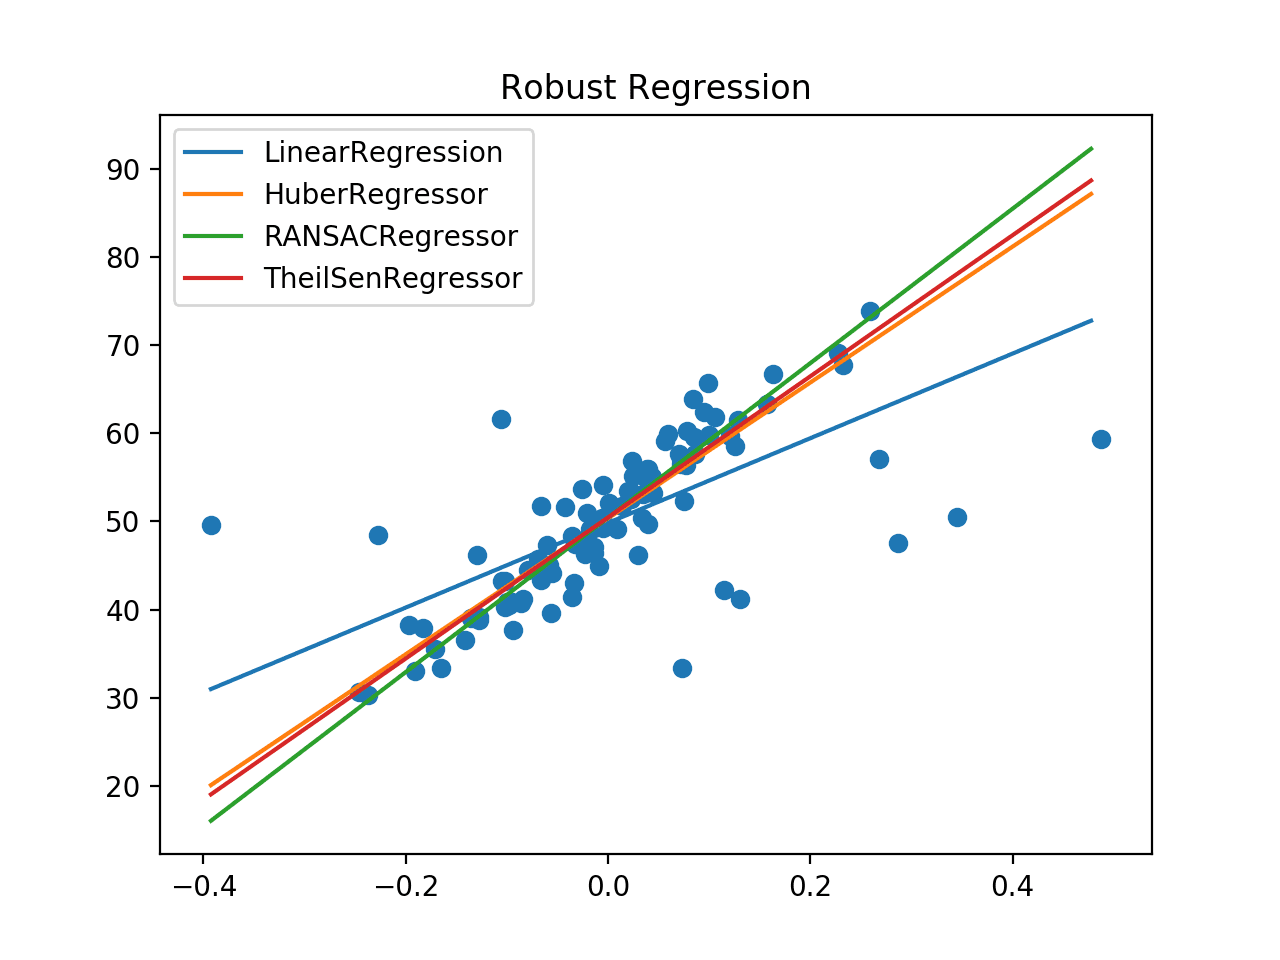
\includegraphics[width=0.9\textwidth]{imagenesResumen/ComparacionRegresiones.png}
    \caption{Diferentes tipos de regresiones. Notar como la lineal (sin ser robusta) se desvía de lo esperado.}
\end{figure}

\newpage

\section{Redes Neuronales}
\begin{itemize}
    \item Basado en neuronas con conexiones con distinta intensidad.
    \item Se activa una neurona cuando recibe suficiente estimulo de las conexiones entrantes.
    \item El primer modelo que surgió fue el Perceptron, a partir de varias entradas daba una salida con una función de activación.
    \item Tienen también una variable Bias, la cual indica que tan fácil es que devuelva 1 la neurona.
    \item El Perceptron funcionaba para casos lineales. \textit{Ej. OR, AND}. 
    \item Unir varios Perceptron hace que actúen como si fuera uno solo.
    \item La solución, fue utilizar una función de activación no lineal. \textit{Función Sigmoidea}. Esta función es aplicada al resultado de la ecuación.
\end{itemize}

Para entrenar una red era necesario poder ajustar los pesos y bias. Esto se hace encontrando los mejores valores de cada uno, y se va consiguiendo a medida que se va reduciendo una función de costo. \textit{Ej. funciones de costo: MSE para regresión, Binaria para clasificación}. Gracias a esta función de costo, ahora la red sabe cuando se equivoco. 

Le falta saber como actualizar los pesos. Esto se consigue utilizando el descenso del gradiente, que apunta a la dirección en la cual la función crece mas rápido. Esta velocidad con la que cambia se conoce como \textit{learning rate}. Si es muy alto puede ir hacia algún mínimo local, si es bajo puede no moverse.

Para cuando se tiene mas de una capa, se utiliza Back Propagation, ya que una neurona depende de los valores de las activaciones de las neuronas de la capa anterior. Con esto se busca modificar las activaciones anteriores para conseguir minimizar aun mas la función de costo.

\begin{figure}[!htb]
    \centering
    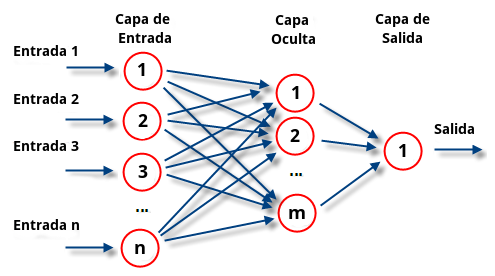
\includegraphics[width=0.9\textwidth]{imagenesResumen/RedNeuronal.png}
    \caption{Modelo de red neuronal.}
\end{figure}

\subsubsection*{¿Que necesita la red?}
\begin{itemize}
    \item Son necesarias tantas neuronas de salida como cantidad de clases a predecir.
    \item La arquitectura, la cantidad de neuronas y la cantidad de capas.
    \item Funciones de activación. \textit{Ej. Sigmoidea, RELU, Softmax}
    \item Optimizadores que determinen como modificar los pesos.\textit{SGD (descenso del gradiente), RMSProp, Adam}.
    \item Una función de costo que se va a estar minimizando.\textit{MSE, MAE, Cross Entropy}.(Depende del problema)
\end{itemize}

Todas estas configuraciones dependen del problema. 

\begin{figure}[!htb]
    \centering
    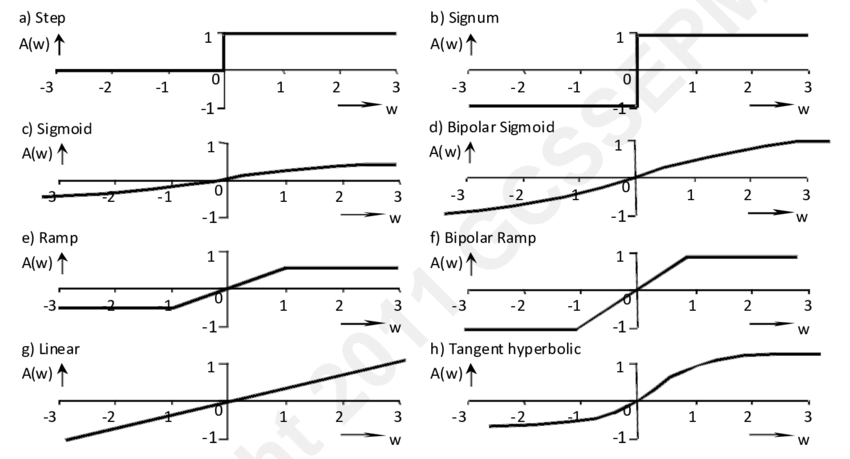
\includegraphics[width=0.8\textwidth]{imagenesResumen/FuncionesActivacion.png}
    \caption{Diferentes funciones de activación.}
\end{figure}

\subsubsection*{Métodos de regularización}
\begin{itemize}
    \item L1, L2, Elastic Net: Penalizan el valor de los pesos de la red.
    \item Dropout: Apaga activaciones aleatoriamente durante el entrenamiento. Esto evita que la red no dependa de unas pocas neuronas.
    \item Early Stopping: Evita el sobreajuste parando el entrenamiento a partir de cierto tiempo.
    \item Data Augmentation: Agrega datos usando los que ya se tienen. (Aplica transformaciones). \textit{Ej. Imagen de un gato, se rota, sigue siendo un gato.}
\end{itemize}

\begin{figure}[!htb]
    \centering
    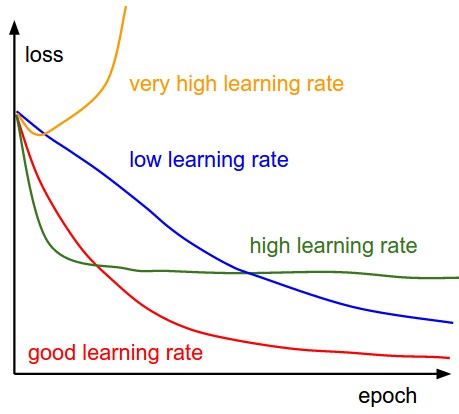
\includegraphics[width=0.8\textwidth]{imagenesResumen/EjemplosEntrenamiento.jpeg}
    \caption{Ejemplos de entrenamiento de una red.}
\end{figure}


\newpage

\section{PLN : Procesamiento del Lenguaje Natural}
Área enfocada a procesar y entender el lenguaje humano. Tiene un montón de usos. \textit{Ej. Traducciones, modelado de tópicos, clasificación de texto, generador de texto...}

\subsection{Enfoques}

\begin{itemize}
    \item Basado en reglas. Busca expresiones regulares, trata de encontrar si un texto cumple con determinadas características.
    \item Modelos probabilísticos. Son clasificadores lineales. Maximizan el likelihood
    \item Deep Learning. Son redes neuronales recurrentes o convolucionales.
\end{itemize}

\subsection{Semantic Slot Filling}
Es una tecnica que asigna categorías semánticas a distintas partes de un texto. Permite que el programa entienda mejor que hacer. Una forma de encararlo es con gramáticas libres de contexto.\textit{Ej. Puede ser Show me..., I want..., Can i see... }.

Los problemas con esta técnica son:
\begin{itemize}
\item Que debe de hacerse manualmente y hay que escribir todas las reglas. Estas son definidas por el humano.
\item Como funciona la técnica, se consigue un presicion alto pero un recall bajo. 
\item Es necesario un corpus de entrenamiento que tenga asignado para cada set de palabras su correspondiente categoría semántica.
\item Requiere de un proceso de feature engineering, ya que hay que preguntarse si las palabras están en mayúscula, cual es el siguiente slot, ...
\item En Deep Learning hay que usar un corpus de datos aun mas grandes.
\end{itemize}

\subsection{Pre-procesamiento}
\subsubsection*{Tokenización}
El texto tiene distintas formas de verse, como caracteres, palabras, frases, oraciones,...

Para hacer esto, podemos utilizar 'Tokens' \textit{Ej. Espacios, comas, cualquier unidad útil para separar}. En otros lenguajes esto se queda corto.

\subsubsection*{Normalización}
Se busca reducir la dimensionalidad. \textit{Ej. Lobos puede pasar a ser Lobo directamente, no nos interesaría el plural.}

Para esto tenemos 2 formas distintas de trabajarlo.
\begin{itemize}
    \item Stemming: Elimina sufijos y prefijos. Trata de llevar la palabra a la raiz.
    \textit{ Ej.
    \begin{itemize}
        \item Feet $\Rightarrow$ Feett
        \item Wolves $\Rightarrow$ Wolv
        \item Talked $\Rightarrow$ Talk
    \end{itemize}
    }
    
    
    \item Lematización: Realiza un análisis morfológico y de vocabulario. 
    \textit{ Ej.
    \begin{itemize}
        \item Feet $\Rightarrow$ Foot
        \item Wolves $\Rightarrow$ Wolf
        \item Talked $\Rightarrow$ Talk
    \end{itemize}
    }
\end{itemize}

\subsubsection*{Extracción de información}
Busca organizar la información de manera útil. Distribuirla de forma precisa para el modelo.

\subsubsection*{Name Entity Recognition}
Busca reconocer y clasificar el texto en categorias.

\textit{Ej. \underline{Ana} se recibió de \underline{ingeniería informática} en la \underline{UBA}.}

\subsubsection*{Colocaciones}
Son frases compuestas por mas de una palabra. \textit{Ej. Buenos Aires}

\subsection{Feature Extraction}
\subsubsection*{Bag of Words}
Cuenta la cantidad de ocurrencias de un token en el texto. El objetivo que tiene es buscar palabras distintivas. \textit{Ej. Excelente, buenísimo,...}

Por cada token se crea una columna de características y se va contando.

Los problemas con esta forma, es que se pierde el orden, que los contadores no están normalizados, y que se tiene una alta dimensionalidad.

Una posible solución es contar de a pares de tokens, pero esto hace que crezca aun mas la dimensionalidad.

\subsubsection*{Soluciones}
Eliminar N-Gramas. Estos serian los de alta frecuencia y los de baja. \textit{Ej. y, o, algún nombre}. El objetivo es quedarse con las palabras que tienen una frecuencia media.


\subsubsection*{TF-IDF}
Se puede usar para una mejora de Bag of Words remplazando a los contadores. Al aplicarlo habria que normalizar cada fila.
\begin{itemize}
\item $TF(t,d)$ - Cuenta la frecuencia de un termino t en el documento d.
\item $IDF(t,D)$= log( $\frac{|D|}{Ocurrencias De t} $) - Cantidad total de documentos en los que aparece un termino. (Inverse Document Frequency)
\item $TF-IDF(t,d,D) = IDF \cdot TF$
\end{itemize}


\subsection{Hipotesis distribucional}
Se asume que la semántica de una palabra esta determinada por el contexto en el que aparece. Esto significaría que se puede obtener el significado de las palabras si las resumimos en los contextos en las cuales aparecen


\subsection{Word2Vec}

Es una forma por la cual se agrupan palabras. Si las palabras tienen significados similares debe de significar que están en espacios vectoriales cercanos. (Esto incluso permite que se puedan realizar operaciones con ellas. \textit{Ej. $Rey - Hombre + Mujer = Reina$})

El objetivo que tiene es entrenar una red neuronal con las palabras del texto, de forma tal de que dada una palabra, nos diga la probabilidad de que cada palabra del vocabulario sea su vecina. (Entrenamos la red y nos quedamos con los pesos de la capa ocula, los 'word vectors')

\textit{Window size}: parámetro que determina el numero de palabras que define un contexto.

La desventajas que tiene este modelo es que no puede trabajar con palabras que no conoce. 

\subsection{FastText}
Mejora de Word2Vec. Para esto trata a las palabras como n-gramas. \textit{Ej. n=2, Hola se representa como Ho,ol,la. Hola se interpreta como la suma de esos 3 n-gramas}. Con este cambio el modelo es capaz de generar embeddings de palabras que no habia visto durante el entrenamiento.

El problema que trae este cambio, es que modelarlo trae un crecimiento de dimensionalidad y memoria enorme. \textit{Ej. 'Se ha visto que para un tamaño de corpus de 50 millones de palabras únicas, el tamaño de RAM requerido puede ser de hasta 256 GB de RAM.'}

Para evitar que se pase, esta limitado en la cantidad máxima de palabras (30 millones). Si se esta alcanzando el limite empieza a hacer remplazos (podas).

La implementación de este modelo esta hecha en C++, por lo que funciona rápidamente debido a la buena optimización de Threads que tiene.


Otros ejemplos similares son Bert y GPT-3.

\newpage

\section{Redes Convolucionales}
Tipo especial de red que se usa para problemas abstractos o difíciles de explicitar. Se basan en ir detectando conceptos e ir resolviendo. Empieza con capas simples y va llegando a las complejas Es muy útil para la clasificación de imágenes.

\begin{figure}[!htb]
    \centering
    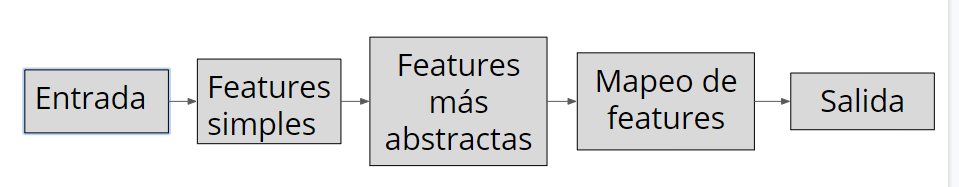
\includegraphics[width=0.9\textwidth]{imagenesResumen/RedesConvolucionalesSistema.PNG}
    \caption{Sistema de trabajo de estas redes.}
\end{figure}

Tiene distintos usos:
\begin{itemize}
    \item Clasificación
    \item Localización
    \item Detección de objetos
    \item Segmentación
\end{itemize}

\begin{figure}[!htb]
    \centering
    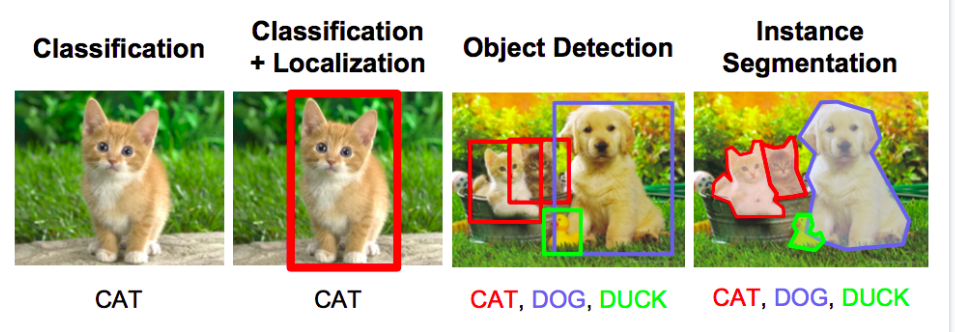
\includegraphics[width=0.9\textwidth]{imagenesResumen/TiposDeUsosRedesConvolucionales.PNG}
    \caption{Ejemplos con algunos de los usos posibles.}
\end{figure}

\begin{itemize}
    \item A medida que se avanza, las capas mas profundas implican conceptos mas complejos.
    \item Se llaman redes convolucionales porque aplican la operación de convolución. \href{https://i1.wp.com/datasmarts.net/es/wp-content/uploads/2018/11/full_padding_no_strides_transposed.gif?resize=264\%2C300&ssl=1}{Gif}
    \item Las redes neuronales comunes no escalan bien en este tipo de problema.
\end{itemize}

\subsection*{Arquitectura}
Las redes estas tienen 2 tipos de capas:
\begin{itemize}
    \item Classification layers: Son neuronas que se conectan con todo el volumen de entrada. (Capa densa comun)
    \item Feature extraction layers: Formadas por capas de convolucion y de filtros.
\end{itemize}

En las capas de convolución se aplican filtros(o kernel) también. Estos filtros reducen la dimensionalidad y tienen sus parámetros que son aprendidos en el entrenamiento. \textit{Ej. \href{https://developers.google.com/machine-learning/practica/image-classification/images/maxpool_animation.gif?hl=es}{MaxPool}, se queda con el valor mas alto}.

\begin{figure}[!htb]
    \centering
    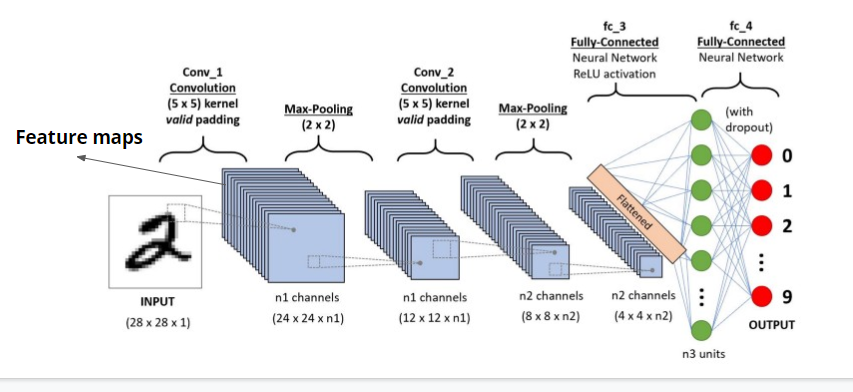
\includegraphics[width=0.9\textwidth]{imagenesResumen/ArquitecturaRedConvolucional.PNG}
    \caption{Arquitectura de la red}
\end{figure}

En los filtros hay que tener en cuenta 3 propiedades:
\begin{itemize}
    \item Stride: Determina los pasos del filtro.
    \item Padding: Hace el rellenado de la imagen.
    \item Depth Volume: Determina la profundidad.
\end{itemize}

Estas redes tienen también métodos de regularización. Los ya vistos en \ref{regularizaciones}.

\newpage

\section{Redes Sociales}
\begin{itemize}
    \item Tienen un crecimiento exponencial.
    \item Son importantes.
    \item Ubicuas.
    \item Modelan distintas cosas.
    \item Crecientes, siempre estuvieron. A partir de la globalización fue exponencial.
    \item Creció la capacidad de mapearlas y estudiarlas.
\end{itemize}

\subsection{¿En cuales participamos?}
\begin{itemize}
    \item Sociales
    \begin{itemize}
        \item Reales: Familia, amigos, trabajo...
        \item Virtuales: Twitter, Facebook,...
    \end{itemize}
    \item Tecnológicas: Internet
    \item De información: www.
    \item De transporte, comercio...
    \item Neuronas
\end{itemize}

\subsection{¿Que modelamos?}
\begin{itemize}
    \item Conectividad
    \item Comportamiento, interacciones
    \item Evolución
\end{itemize}

\subsection{¿Quienes se ocupan?}
Tienen distintas escalas, distintas visiones
\begin{itemize}
    \item Estructura, complejidad, sistemas conectados $\Longleftrightarrow$ Computación, matemática, física
    \item Estratégico $\Longleftrightarrow$ Economía, psicología
    \item Grupales, agregado $\Longleftrightarrow$ Sociología
    \item Sistemas gigantes, Big data $\Longleftrightarrow$ Computación
\end{itemize}

Cada uno tiene sus teorías subyacentes, de grafos, juegos, y redes.

\subsection{Análisis de las redes sociales}
\begin{itemize}
    \item Diferencias entre amigos y conocidos. \textit{Ej. Cambio de trabajo. Mas probable que venga de conocidos. Actúan como puentes entre grupos}
    \item Principio de clausura triadica.
    \item Mundo pequeño: 6 niveles de separación. \textit{Ej. Carta a Boston}.
\end{itemize}

\subsection*{Puente}
\begin{itemize}
    \item Eje cuya eliminación desconecta un grafo.
    \item En los mundos pequeños (grafos muy conexos) son poco comunes.
\end{itemize}

\subsubsection*{Puentes Locales}
Su eliminación no desconecta al grafo, pero aumenta el recorrido.

\subsection*{Homofilia}
\begin{itemize}
    \item Los nodos conectados tienden a ser parecidos.
    \item \textit{Ej. Amigos con gustos parecidos}.
    \item 'Te metes en la burbuja'.
    \item Existe la homofilia inversa.
    \item Se puede medir al comparar cuanto se parecen los ejes de los grafos.
\end{itemize}

\subsection*{Relaciones +/-}
\begin{itemize}
    \item Amigo o enemigo
    \item Existen 4 tipos de triángulos. Ver la imagen \ref{triangulos}
\end{itemize}

\begin{figure}[!htb]
    \centering
    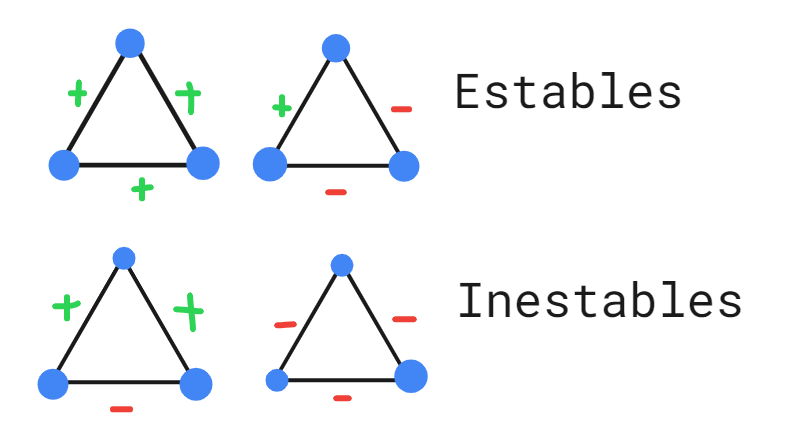
\includegraphics[width=0.6\textwidth]{imagenesResumen/Triangulos.png}
    \caption{Los 4 tipos de triángulos posibles. Los + representan a los 'amigos' y los - a los 'enemigos'.}
    \label{triangulos}
\end{figure}


Hay un balanceo estructural si todos los triángulos de una estructura son estables. Caso contrario se tiende a romper y generar problemas.

\newpage

\section{Aprendizaje por refuerzo}
\textit{
Un \underline{agente} (similar a modelo) tiene sensores para observar el \underline{estado} de su entorno. Con el cual puede hacer \underline{acciones} para alterar ese estado. Estas acciones conllevan una \underline{recompensa} numérica.
}

Estas recompensas que el agente recibe vienen con cierta demora. Ya que hay que discernir entre cuales fueron las meritorias.

\begin{figure}[!htb]
    \centering
    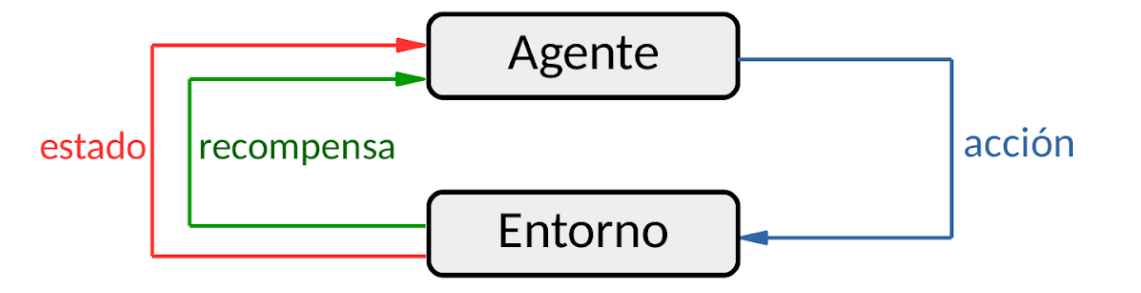
\includegraphics[width=0.9\textwidth]{imagenesResumen/AprendizajeRefuerzo.PNG}
    \caption{Sistema de aprendizaje por refuerzo.}
\end{figure}


\subsection{Q-Learning}
Algoritmo con el cual se controla el aprendizaje. Se busca aprender la función óptima fruto de la política óptima.

Se le indica un $\alpha$ (learning rate) que indica que tanto aprende. Si se aumenta mucho puede llevar a un mínimo local. Si es muy bajo el agente no se va a estar moviendo.

¿Como determinar la acción en base al estado? Hay que buscar un equilibrio entre la explotación y la exploración. Hay 2 estrategias para esto.

\begin{itemize}
    \item $\epsilon-greedy$ Con la probabilidad $\epsilon$ elegimos al azar uno, y con 1-$\epsilon$ elegimos la acción que mejor conocemos.
    \item $\epsilon-first$ Elegimos al azar cierta cantidad de casos (1-$\epsilon$)\%, y después el que mejor conocemos ($\epsilon$)\%. 
\end{itemize}

Este algoritmo (Q-Learning) tiene los problemas de que no aprende la noción de estados similares y de que a nivel practico no escala bien, se vuelve intratable (no es el caso teórico). Una alternativa para evitar esto, es aproximar la función Q del algoritmo con una red neuronal de convolución.

\subsubsection*{Algoritmo}
\begin{enumerate}
    \item Inicializar $Q(s,a)$
    \item Inicializar $s$
    \item Elegir la acción $a$ en $s$ y ejecutarla
    \item Observar la recompensa $r$ en el nuevo estado $s'$
    \item Repetir a partir de 2 hasta que el estado $s$ sea terminal.
\end{enumerate}

Gif mostrando un \href{http://ikuz.eu/wp-content/uploads/2015/02/breakout.gif}{ejemplo}. Este seria el caso ya entrenado, donde lo que aprendió es a mover la pelota para el fondo del juego, de forma tal de que rebote sola y limpie el mapa. Al comienzo apenas responde.

\newpage

\section{Ética y moral en ML}
\subsection{¿Por que discutirlo?}
\begin{itemize}
    \item Impacto económico
    \begin{itemize}
        \item Hay mucha materia prima (datos)
        \item Mucha capacidad de procesamiento y almacenamiento
        \item Centrales de datos
    \end{itemize}
\end{itemize}

\subsection{Posicionamientos}
\begin{itemize}
    \item Optimista
    \begin{itemize}
        \item No confinar o intentar controlar a la IA.
        \item Enseñarle los valores humanos.
        \item Hay que tener un planteo simbiótico.
    \end{itemize}
    \item Pesimista
        \begin{itemize}
        \item Que nos va a pasar y atentar contra nosotros.
    \end{itemize}
    \item Realistas
        \begin{itemize}
        \item Es falso el desarrollo exponencial de la IA.
        \item Es falso que constituyen un peligro.
        \item Los progresos son lineales.
    \end{itemize}
\end{itemize}

\subsection{Usos}
La IA tiene muchos usos. Estos varían desde asistentes personales, redes de transporte, buscadores, publicidad, etc. 

\subsection{Preguntas a hacerse}
\begin{itemize}
    \item ¿Quien guarda la información?
    \item ¿Violación de derechos?
\end{itemize}

Hay que hacer los problemas y cuestiones éticas explícitos. Evitar los sesgos y las violaciones de privacidad.

Estas cuestiones no pueden quedar en pasarle la responsabilidad al usuario directamente, ya que el usuario es el ultimo en la cadena de desarrollo. Las empresas disponen de una mayor cantidad de herramientas para tratar los temas.

Una forma es incorporar las cuestiones éticas en los métodos de diseño, y alinearlos a los valores humanos. El tema que surge es: ¿Cuales? ¿Quien los decide?  ¿Con que interpretación? Son cuestiones que hay que definir. Dejar de forma clara que es desleal y que no.

\subsection{Teorías éticas}
\begin{itemize}
    \item Meta-ética: Estudia los principios. \textit{Ej. Objetivismo vs Relativismo}
    
    \item Ética Normativa: La que genera reglas y nos interesa en \textit{Machine Learning}
    
    \item Ética Aplicada: Trata las situaciones sociales. \textit{Ej. Derechos de animales, eutanasia...}
\end{itemize}

\subsection{Ética Normativa}
\begin{itemize}
    \item Ética de la virtud: Busca la moralidad de una acción. Hábitos vs Reglas.
    \item Ética consecuencialista: Evalúa el resultado.
    \item Ética deontológica: Propone evaluar la moralidad de una acción
\end{itemize}


Tiene 2 enfoques:
\begin{itemize}
    \item Top-Down: Se basa en el deber, toma la teoría previa y la deriva.
    \item Bottom-Up: Se intenta capturar la teoría a partir de la observación. Aprendizaje, emoción.
\end{itemize}

Ambas tienen el problema del marco. El cual se basa en el impacto en el contexto. Se puede medir que sucede en el local, pero no en los colaterales.

\end{document}

